\documentclass[a4paper,12pt]{report}

% Pacchetti
\usepackage[utf8]{inputenc}
\usepackage[T1]{fontenc}
\usepackage[italian]{babel}
\usepackage{amsmath,amssymb,amsfonts}
\usepackage{graphicx}
\usepackage{csquotes}
\usepackage{float}
\usepackage{caption}
\usepackage{booktabs}
\usepackage{listings}
\usepackage{tikz}
\usepackage{enumitem}
\usepackage{tabularx}
\usepackage{theorem}

% FONT LEGGIBILI + SPAZIATURA
\usepackage{newpxtext}       % Palatino moderno
\usepackage{newpxmath}       % Matematica Palatino
\usepackage{microtype}       % Ottimizzazione micro-tipografica
\usepackage{setspace}        % Gestione interlinea
\onehalfspacing              % Interlinea 1.5

% Hyperref (caricare per ultimo)
\usepackage{hyperref}

\title{Analisi Comparativa di KAN, MLP, Random Forest e XGBoost con Tecniche di Ottimizzazione}
\author{Martin Tomassi \\ Università di Bologna \\ Corso di Laurea in Ingegneria e Scienze Informatiche}
\date{Settembre 2025}

\begin{document}
	
	\maketitle
	
	\tableofcontents
	
	\chapter{Introduzione}
	La presente tesi si propone di analizzare, confrontare e valutare diverse architetture di Machine Learning: le Kolmogorov–Arnold Networks (KAN), i Multi-Layer Perceptron (MLP), le Random Forest e XGBoost. \\
	L’obiettivo principale è quello di fornire, da un lato, un’analisi teorica esaustiva di ciascun modello, includendo i fondamenti matematici e le architetture; dall’altro, valutare sperimentalmente le prestazioni dei modelli su tre casi di studio: regressione sulle emissioni di automobili, classificazione dell’inquinamento atmosferico (PM2.5) e riconoscimento di immagini mediante CNN abbinate a MLP e KAN. \\
	Oltre allo studio comparativo dei modelli, la tesi include un’ampia indagine sui metodi di Hyperparameter Tuning: Grid search, Random search, Bayesian optimization e Genetic algorithms, selezionati in base ad uno studio preliminare di confronto. \\
	A completamento, sono stati condotti due studi di ablazione post-training per ogni caso di studio:
	\begin{itemize}
		\item \textbf{L1 Pruning} per KAN e MLP.
		\item \textbf{Ensemble Pruning} dove:
		\begin{itemize}
			\item \textbf{Rank-Based Pruning} per Random Forest.
			\item \textbf{Cumulative Pruning} per XGBoost.
		\end{itemize}
	\end{itemize}
	
	\chapter{Kolmogorov--Arnold Networks (KAN)}
	
	\section{Fondamenti matematici}
	
	\subsection{Enunciato del teorema di Kolmogorov--Arnold}
	Il teorema di Kolmogorov--Arnold (KART) stabilisce che ogni funzione continua multivariata, su un intervallo compatto, può essere rappresentata come una combinazione di somme di funzioni univariate. In forma esplicita: per una funzione continua \(f:[0,1]^n \to \mathbb{R}\) esistono funzioni continue univariate \(\phi_{q,p}\) e \(\Phi_q\) tali che
	\[
	f(x_1,\dots,x_n)=\sum_{q=1}^{2n+1}\Phi_q\!\Biggl(\sum_{p=1}^n \phi_{q,p}(x_p)\Biggr),
	\]
	per \(q=1,\dots,2n+1\). In altre parole, ogni funzione multivariata può essere ricondotta a combinazioni di funzioni monovariate tramite opportune funzioni interne \(\phi_{q,p}\) ed esterne \(\Phi_q\).
	
	Questo risultato mostra che l'unica vera interazione tra le variabili, nella rappresentazione data, è la somma: tutte le altre dipendenze possono essere "scomposte" in funzioni di una sola variabile.
	
	\subsection{Sulla natura "non costruttiva" delle dimostrazioni}
	Le dimostrazioni originali del KART, eseguite da Kolmogorov nel 1957 e successivamente Arnold nel 1967, sono di natura esistenziale: garantiscono l'esistenza delle funzioni \(\phi_{q,p}\) e \(\Phi_q\), ma non forniscono una procedura esplicita o una formula chiusa per costruirle. Pertanto il teorema è fondamentale dal punto di vista teorico ma, senza ulteriori risultati costruttivi, ha limitata utilità pratica per la costruzione diretta di architetture neurali basate su tali funzioni, spingendo i ricercatori a privilegiare le reti neurali multistrato (MLP) che, pur con i loro limiti, erano più facili da implementare.
	
	\section{Architettura delle KAN}
	
	\begin{figure}[H]
		\centering
		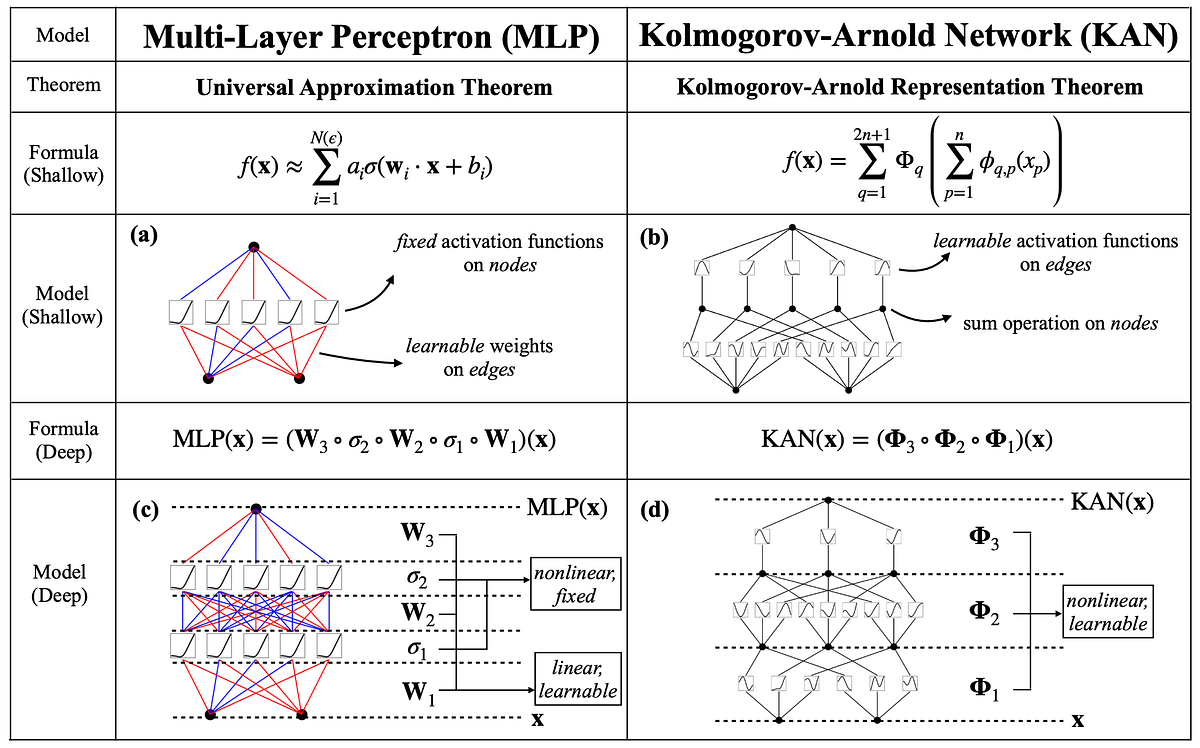
\includegraphics[width=1.0\textwidth]{img/KANvsMLP.png}
		\caption{Confronto schematizzato tra un Multi-Layer Perceptron (MLP) tradizionale e una Kolmogorov–Arnold Network (KAN).}
		\label{fig:KANvsMLP}
	\end{figure}
	Una Kolmogorov–Arnold Network (KAN) è strutturalmente simile ad una rete feedforward completamente connessa, simile ad una MLP, ma differiscono in modo sostanziale nell'uso delle funzioni di attivazione: ogni arco (collegamento) tra i neuroni di strati consecutivi porta con sé una funzione univariata parametricamente definita (spesso una B-spline), anziché un peso scalare come nei MLP. Ciascun neurone di uno strato riceve gli output dei collegamenti in ingresso e calcola semplicemente la somma di tali output; non vi sono pesi lineari né attivazioni non lineari aggiuntive sui nodi stessi.
	
	Il modello generale si descrive così: se lo strato $(\ell-1)$ ha $d_{\ell-1}$ neuroni e lo strato $\ell$ ne ha $d_\ell$, allora esiste una matrice di funzioni unidimensionali $\{f^{(\ell)}_{ij}\}_{i=1,\dots,d_{\ell-1}}^{j=1,\dots,d_\ell}$ tale che, dati gli output degli $d_{\ell-1}$ neuroni precedenti $x_i^{(\ell-1)}$, l’uscita $x_j^{(\ell)}$ del $j$-esimo neurone del livello $\ell$ è: 
	\[
	x_j^{(\ell)} \;=\; \sum_{i=1}^{d_{\ell-1}} f^{(\ell)}_{ij}\bigl(x_i^{(\ell-1)}\bigr)\,.
	\] 
	In forma matriciale si può scrivere $x^{(\ell)} = f^{(\ell)}(x^{(\ell-1)})$, dove $f^{(\ell)}$ è l’insieme delle funzioni collegamento per quello strato. L’output complessivo della KAN è quindi dato dalla composizione degli strati successivi: 
	\[
	y \;=\; x^{(L)} 
	= f^{(L)}\bigl(f^{(L-1)}(\dots f^{(1)}(x^{(0)})\dots)\bigr)\!,
	\] 
	dove $x^{(0)}$ è il vettore di input della rete. Questa architettura "fonde" le trasformazioni lineari e non-lineari in un'unica funzione $f_{ij}$ per ogni arco, permettendo alla rete di apprendere la forma esatta della funzione di attivazione necessaria per ogni connessione.
	
	Si noti che un MLP applica funzioni di attivazione predefinite (ReLU, sigmoid, ecc.) sui singoli neuroni e moltiplica gli input per pesi scalari; al contrario, una KAN utilizza funzioni parametriche sugli archi e non applica nessuna attivazione aggiuntiva sui neuroni.
	
	\subsection{Tipologie di funzioni di attivazione usate}
	
	Le funzioni di attivazione utilizzate nelle KAN sono funzioni univariate parametriche scelte in modo da poter apprendere flessibilmente la forma. Nell’implementazione classica proposta da Liu et al. (2024), queste funzioni sono rappresentate come B-spline (polinomi a tratti), una scelta che offre un buon compromesso tra flessibilità locale e complessità di calcolo. Ciascuna funzione su un collegamento è quindi $f_{ij}(t) = t + g_{ij}(t)$, dove la parte $g_{ij}(t)$ è espressa come una combinazione lineare di spline di ordine tipicamente basso (ad esempio di grado 3) su un numero predefinito di nodi. Tale formulazione con residuo lineare migliora l’ottimizzazione: il termine lineare garantisce un comportamento iniziale affine, mentre il termine spline introduce la non linearità appresa. Un altro aspetto importante è la spline grid, ovvero la suddivisione dell'asse degli input in nodi che determinano dove iniziano e finiscono gli intervalli di ogni polinomio.
	
	In generale, oltre alle B-spline, si potrebbero utilizzare anche altre famiglie di funzioni unidimensionali parametrizzate. Ad esempio, è possibile usare polinomi di Chebyshev o altre basi ortogonali a seconda del problema specifico. Le reti KAN sono infatti in grado di adattarsi a diverse funzioni di attivazione: i coefficienti della spline (o di qualunque base scelta) sono parametri addestrabili della rete, aggiornati durante il training.
	
	\subsection{Leggi di scaling e la "curse of dimensionality"}
	
	Come suggerito dal teorema matematico di riferimento, le KAN godono di proprietà di approssimazione universale analoghe ai MLP tradizionali. In particolare, se $f$ è una funzione continua su un dominio compatto, il teorema di Kolmogorov–Arnold garantisce che esista una KAN (di profondità 2 e larghezza $\mathcal{O}(n)$) che la rappresenta esattamente. Pertanto, per ogni tolleranza $\epsilon>0$ esiste un modello KAN sufficientemente ampio che approssima $f$ entro errore $\epsilon$, cioè $\|f_{\text{KAN}}-f\|<\epsilon$.

	Quindi le KAN possono superare il problema legato al "curse of dimensionality". Sotto l'ipotesi che la funzione da apprendere abbia una struttura additivo-composizionale, l'errore di approssimazione di una KAN diminuisce in modo indipendente dalla dimensione dell'input, superando il problema. Questo si traduce in leggi di scaling neurali più veloci rispetto alle MLP.
	
	Mentre per le MLP il numero di neuroni necessario per ottenere una data precisione può crescere esponenzialmente con la dimensione dell'input, teoricamente, le KAN riescono a ottenere la stessa accuratezza con molti meno parametri. Questo perché le KAN, a differenza delle MLP, apprendono non solo la struttura composizionale (la relazione tra le variabili) ma anche le funzioni univariate con grande precisione, grazie all'uso delle spline.
	
	\section{Funzionamento operativo}
	
	\subsection{Calcolo del mapping input–hidden–output}
	
	Nel funzionamento operativo di una KAN, i dati scorrono in avanti attraverso gli strati esattamente come in una normale MLP, ma usando le funzioni di attivazione sugli archi. Dato un vettore di input $x^{(0)}$, il calcolo procede layer dopo layer: per ciascun neurone nel primo strato nascosto si valuta la somma delle funzioni dei collegamenti in ingresso applicate alle componenti di $x^{(0)}$, ottenendo $x^{(1)}$ e così via. Al livello successivo si ripete lo stesso procedimento prendendo $x^{(1)}$ come input, e così via fino allo strato di output. Formalmente, ogni layer $\ell$ esegue la trasformazione $x^{(\ell)} = f^{(\ell)}(x^{(\ell-1)})$, e l’output finale è $y = x^{(L)}$. Grazie al fatto che tutte le operazioni (applicazione delle funzioni univariate e somme) sono differenziabili, il modello complessivo è addestrabile tramite backpropagation. Questo significa che i coefficienti delle funzioni di attivazione (ad esempio, delle spline) possono essere ottimizzati tramite discesa del gradiente, minimizzando una funzione di perdita, allo stesso modo di quanto avviene in un MLP.
	
	\subsection{Processo di training e calcolo dei pesi}
	
	Il training di una KAN segue la procedura standard di addestramento supervisionato con discesa del gradiente. Si assume un insieme di dati di addestramento $(x,y)$ ed una loss (ad esempio, l’errore quadratico medio per problemi di regressione), quindi si aggiornano iterativamente i parametri delle funzioni di attivazione. Nelle KAN, i "pesi" da addestrare sono i coefficienti che definiscono le funzioni unidimensionali sui collegamenti. Per esempio, una spline di ordine 3 su $r$ intervalli ha $r+3$ coefficienti; ciascun coefficiente è un parametro della rete. È prassi includere un termine base lineare (di solito la stessa identità), come in 
	\[
	f_{ij}(t) = t + g_{ij}(t)\,, 
	\]
	dove $g_{ij}$ è la spline addestrabile. Questo facilita la convergenza iniziale.
	
	Durante l’ottimizzazione si può anche aggiornare adattivamente la griglia di definizione delle spline, così da coprire automaticamente i nuovi intervalli di attivazione che emergono durante il training (grid extension). In pratica, ogni volta che un valore di attivazione supera la griglia corrente, si estende dinamicamente il supporto della spline per mantenere il dominio di apprendimento adeguato. In sintesi, il flusso di calcolo è identico ad un MLP: si effettua forward pass, si calcola la loss, e poi si retropropaga l’errore calcolando gradienti rispetto ai coefficienti delle funzioni $g_{ij}$.
	
	\subsection{Complessità computazionale}
	
	Dal punto di vista parametrico, una KAN può avere un numero di parametri superiore rispetto ad un MLP di dimensioni simili. Ad esempio, supponiamo una KAN con $L$ strati, ciascuno di larghezza $m$, che usa spline di ordine $p$ su $r$ intervalli. Allora il numero totale dei parametri della rete KAN cresce come $\mathcal{O}(L\,m^2\,p\,r)$, mentre un MLP con $L$ strati e larghezza $m$ avrebbe circa $\mathcal{O}(L\,m^2)$ pesi scalari. In teoria quindi le KAN appaiono meno efficienti in termini di numero di parametri. Tuttavia, empiricamente si osserva che spesso basta una KAN con dimensioni molto più piccole per eguagliare le prestazioni di un MLP molto più grande.
	
	Dal punto di vista computazionale, l’impiego di funzioni parametriche sugli archi comporta un overhead rispetto alle semplici moltiplicazioni peso-input di un MLP. In pratica, valutare una B-spline su ogni collegamento è più costoso del prodotto scalare in un MLP, soprattutto se la rete è profonda o le spline sono molto finemente discretizzate (cioé utilizzano un numero elevato di punti di controllo). Quindi, l'addestramento di una KAN, può essere più lento, con stime che indicano un tempo di training circa 10 volte superiore rispetto alle MLP a parità di condizioni.
	
	\section{Interpretazione e flessibilità locale}
	Uno dei principali vantaggi delle KAN è la loro intrinseca interpretabilità. Poiché ogni arco implementa una funzione univariata ben definita, è possibile visualizzare direttamente le forme delle attivazioni apprese. Questo permette di comprendere i singoli contributi delle variabili di input e, in alcuni casi, di dedurre formule simboliche sottostanti. Le KAN sono state definite "collaboratori" utili per aiutare gli scienziati a riscoprire leggi matematiche e fisiche.
	
	Un altro vantaggio importante è la flessibilità locale che deriva dalla natura delle spline. A differenza delle MLP che usano attivazioni globali (come ReLU o Tanh), una KAN modifica solo una piccola regione di input quando apprende una nuova informazione. Ciò riduce significativamente il rischio di "catastrophic forgetting", un fenomeno in cui l'addestramento su nuovi dati può distruggere le informazioni precedentemente apprese.
	
	\section{Confronto con MLP tradizionali}
	
	\subsection{Architettura a confronto}
	
	Dal punto di vista architetturale, l’architettura di base di una KAN è feedforward e totalmente connessa come quella di un MLP. La differenza fondamentale risiede nel collocamento delle non-linearità e nell’assenza di matrici di pesi lineari. Come abbiamo visto, in un MLP ogni neurone applica una funzione di attivazione fissa (ReLU, sigmoid, ecc.) dopo una combinazione lineare dei suoi input, mentre in una KAN ogni collegamento possiede direttamente una funzione attivazione addestrabile. Di conseguenza, una KAN “fonde” le trasformazioni lineari e non-lineari in un’unica funzione $f_{ij}$ per ogni arco, anziché trattarle separatamente come in un MLP.
	
	In termini pratici, un MLP a $L$ strati alterna operazioni $x \mapsto W x + b$ e $x \mapsto \sigma(x)$, mentre una KAN sostituisce ogni prodotto $W_{ij}x_i$ con $f_{ij}(x_i)$. Questo implica che una KAN può essere visto come un MLP “con pesi che variano in modo non-lineare col valore dell’input”. 
	
	In definitiva, mentre gli MLP hanno architetture fisse con attivazioni prefissate, le KAN introducono una sorta di adattamento interno aggiuntivo: la rete impara direttamente la forma della funzione di attivazione necessaria per ogni connessione. Questo dà alle KAN una capacità di modellare strutture additive-compositive molto esplicite, coerentemente con il teorema di Kolmogorov–Arnold.
	
	\subsection{Vantaggi delle KAN}
	
	\subsubsection{Efficienza parametrica e leggi di scaling} 
	Quando la funzione obiettivo è ben approssimabile tramite somme di funzioni univariate, una KAN può raggiungere livelli di accuratezza comparabili (o superiori) ad un MLP molto più grande, usando un numero di parametri sensibilmente inferiore. In queste situazioni l'errore di approssimazione dipende principalmente dalla risoluzione delle griglie e dall'ordine delle spline, anziché crescere esponenzialmente con la dimensione \(d\) dell'input; ciò produce leggi di scaling più favorevoli e frontiere di Pareto migliori tra complessità ed accuratezza sul training e test.
	
	\subsubsection{Precisione controllabile tramite estensione della griglia}
	Le funzioni univariate nelle KAN sono parametrizzate tramite B-spline definite su una griglia. È possibile aumentare la risoluzione della griglia ("grid extension") per incrementare la precisione in modo controllato: partendo da spline grossolane si possono ottenere spline più fini con una procedura di inizializzazione che conserva la continuità e permette rapide riduzioni della loss senza costi computazionali esponenziali.
	
	\subsubsection{Interpretabilità}
	Poiché ogni arco della rete implementa una funzione univariata esplicita, le forme apprese sono direttamente ispezionabili. Questo consente di riconoscere comportamenti funzionali (lineare, polinomiale, sinusoidale, \ldots) e facilita il collegamento con analisi simboliche o di dominio, oltre a rendere più semplice il debug e la semplificazione del modello.
	
	\subsubsection{Flessibilità locale e robustezza al catastrophic forgetting}
	L'uso di B-spline introduce località nelle rappresentazioni: modifiche ai coefficienti influiscono principalmente su intervalli ristretti dell'input. Tale località si traduce in una flessibilità locale che riduce la tendenza al catastrophic forgetting nei setting di apprendimento sequenziale, rispetto a rappresentazioni globali tipiche delle MLP.
	
	\subsubsection{Rappresentazione precisa di componenti univariate}
	Per compiti scientifici dove la precisione locale è critica, le KAN permettono un'approssimazione fine di componenti univariate che nelle MLP richiederebbe reti molto più ampie o attivazioni progettate ad hoc.
	
	\subsection{Limiti delle KAN}
	
	\subsubsection{Dipendenza dalla struttura composizionale}
	I vantaggi più netti emergono solo se la funzione target è effettivamente vicina a una decomposizione in somme di funzioni univariate. Quando la funzione è intrinsecamente non decomponibile o presenta forti interazioni multivariate, la rappresentazione KAN perde efficacia e può risultare meno efficiente rispetto ad una parametrizzazione densa tipica delle MLP.
	
	\subsubsection{Irregolarità nella rappresentazione di Kolmogorov}
	Il teorema di Kolmogorov–Arnold garantisce l'esistenza di una rappresentazione, ma non la regolarità delle funzioni intermedie \(\varphi_{q,p}\). In casi pratici queste funzioni possono essere non-smooth o altamente oscillanti; per approssimarle con spline possono essere necessarie griglie molto fitte, annullando i vantaggi teorici in termini di parametri e costo computazionale.
	
	\subsubsection{Overhead computazionale e scelta della struttura}
	Parametrizzare ogni arco come funzione spline introduce overhead in memoria ed in tempo di calcolo (valutazione e aggiornamento di B-spline, gestione di griglie differenziate). Inoltre, la scelta automatica della topologia (numero di rami, profondità, risoluzione delle griglie per ciascuna spline) non è banale e richiede procedure di pruning o ricerca strutturale che aumentano la complessità del workflow.
	
	\subsubsection{Sensibilità al rumore e necessità di regolarizzazione}
	In presenza di dati molto rumorosi, una parametrizzazione spline troppo fine tende al sovraffitting locale. È quindi necessario un attento tuning degli iperparametri (ordine della spline, numero di nodi, termine di regolarizzazione, smoothing), e in alcuni casi una MLP ben regolarizzata può mostrare maggiore robustezza.
	
	\subsubsection{Non universalità della superiorità prestazionale}
	Benchè efficaci in molti scenari (function fitting, PDE, continual learning, discovery scientifica), le KAN non garantiscono vantaggi su tutti i task: su dataset di classificazione complessi o domini ad alta complessità multivariata sperimentazioni recenti mostrano che le KAN non sempre superano MLP ottimizzate. È pertanto consigliabile valutare empiricamente il rapporto costo/beneficio sul problema concreto prima di adottare una KAN come soluzione standard.
	
	\section{Applicazioni delle KAN}
	Le reti KAN sono state sperimentate con successo in diversi contesti applicativi, con risultati particolarmente promettenti in scenari dove l'interpretabilità e la precisione sono cruciali.
	
	\begin{itemize}
		\item \textbf{Risoluzione di Equazioni Differenziali Parziali (PDEs)}: le KAN hanno mostrato una notevole superiorità rispetto alle MLP nella risoluzione di PDEs, come dimostrato nel caso di un problema di Poisson. Una KAN a 2 strati di ampiezza ridotta ha raggiunto errori significativamente inferiori rispetto a una MLP molto più grande.
		\item \textbf{Function Fitting e Symbolic Regression}: le KAN eccellono nel "function fitting", ovvero l'approssimazione di funzioni complesse. Sono in grado di identificare e apprendere le strutture composizionali presenti in formule matematiche, come dimostrato con le equazioni di Feynman. Grazie alla loro interpretabilità, le KAN possono essere utilizzate come "collaboratori" nella regressione simbolica, aiutando gli scienziati a (ri)scoprire leggi matematiche.
		\item \textbf{Applicazioni Scientifiche (AI + Science)}: la capacità delle KAN di offrire interpretabilità e precisione le rende candidati ideali per la ricerca scientifica. Sono state usate per studiare problemi come la teoria dei nodi e i confini di transizione di fase nella fisica della materia condensata, fornendo insight che i modelli tradizionali non potevano offrire.
	\end{itemize}
	
	In sintesi, le reti di Kolmogorov-Arnold costituiscono una nuova famiglia di architetture neurali che sfruttano un'importante idea teorica per migliorare l'espressività e l'interpretabilità rispetto alle MLP tradizionali. L'uso di attivazioni parametriche sugli archi permette di catturare efficacemente strutture additivo-composizionali e, quando queste sono presenti, di ottenere migliori prestazioni (in termini di accuratezza ed efficienza parametrica). Allo stesso tempo, rimangono aperte sfide pratiche e teoriche, come l'identificazione automatica della forma ottimale delle KAN e l'estensione efficiente a casi non strettamente additivi, che sono oggetto di ricerca attuale.
	
	\chapter{Multi-Layer Perceptron}
	
	\section{Introduzione}
	Le Multi-Layer Perceptron (MLP) sono una famiglia di reti neurali feedforward composte da unità (neuroni) organizzate in strati: uno strato di input, uno o più strati nascosti e uno strato di output. Ogni neurone in uno strato (eccetto quelli di input) calcola una combinazione lineare degli ingressi seguita dall'applicazione di una funzione di attivazione non lineare. Grazie a queste non linearità, le MLP possono approssimare relazioni complesse tra input ed output e rappresentano uno strumento fondamentale nel Deep Learning per compiti di regressione, classificazione e clustering.
	
	\section{Teorema di approssimazione universale}
	
	\subsection{Enunciato formale}
	Sia \(K\subset\mathbb{R}^n\) uno spazio compatto e sia \(C(K)\) lo spazio delle funzioni continue su \(K\) munito della norma uniforme \(\|\cdot\|_\infty\). Sia \(\sigma:\mathbb{R}\to\mathbb{R}\) una funzione di attivazione che soddisfa una delle seguenti ipotesi:
	
	\begin{enumerate}
		\item[\((A_1)\)] \(\sigma\) è continua e sigmoide, cioè \(\lim_{t\to -\infty}\sigma(t)=a\) e \(\lim_{t\to +\infty}\sigma(t)=b\) con \(a\neq b\) (Cybenko);
		\item[\((A_2)\)] \(\sigma\) è continua e non polinomiale (v.\ Leshno et\,al.). 
	\end{enumerate}
	
	Allora vale il seguente risultato di approssimazione uniforme.
	
	\subsection{Teorema di approssimazione universale}
	Per ogni \(f\in C(K)\) e per ogni \(\varepsilon>0\) esistono un intero \(N\in\mathbb{N}\) (indica il numero di neuroni nello strato nascosto), coefficienti scalari \(c_i\in\mathbb{R}\), vettori \(w_i\in\mathbb{R}^n\) e bias \(b_i\in\mathbb{R}\) tali che la funzione a singolo strato
	\[
	\hat f_N(x) \;=\; \sum_{i=1}^N c_i\,\sigma\bigl(w_i\cdot x + b_i\bigr)
	\]
	soddisfa
	\[
	\|f - \hat f_N\|_\infty \;=\; \sup_{x\in K} \bigl|f(x)-\hat f_N(x)\bigr| \;<\; \varepsilon.
	\]
	In altre parole, lo span delle funzioni elementari (cioè l'insieme di tutte le possibili combinazioni lineari di queste funzioni) \(x\mapsto\sigma(w\cdot x + b)\) è denso in \(C(K)\) rispetto alla norma uniforme. Ciò significa che per ogni funzione continua \(f\in C(K)\) e per ogni \(\varepsilon>0\) esiste una combinazione lineare finita di blocchi attivati da \(\sigma\) (cioè una rete a singolo strato nascosto) che approssima \(f\) uniformemente su \(K\) con errore massimo minore di \(\varepsilon\). Formalmente, la chiusura (nell'\(\|\cdot\|_\infty\)) dello spazio generato dalle funzioni elementari coincide con l'intero \(C(K)\).
	
	\subsection{Significato di \(\sup_{x\in K}\).}
	La notazione \(\sup_{x\in K}\) denota l'estremo superiore di un insieme di reali. Nella norma uniforme
	\[
	\|f-\hat f_N\|_\infty=\sup_{x\in K}|f(x)-\hat f_N(x)|
	\]
	il valore indicato è l'errore massimo di approssimazione su tutto il dominio \(K\). Poiché nel teorema \(K\) è assunto compatto e la funzione \(x\mapsto|f(x)-\hat f_N(x)|\) è continua, l'estremo superiore coincide con il massimo:
	\[
	\sup_{x\in K}|f(x)-\hat f_N(x)|=\max_{x\in K}|f(x)-\hat f_N(x)|.
	\]
	
	\paragraph{Esempio} Se \(K=[0,1]\) e \(f(x)=\sin(2\pi x)\), affermare che esiste \(N\) tale che
	\[
	\sup_{x\in[0,1]}|f(x)-\hat f_N(x)|<0.01
	\]
	significa che con quel numero di neuroni si può costruire \(\hat f_N\) che differisce dalla sinusoide al più di \(0.01\) in ogni punto dell'intervallo \([0,1]\).
	
	\subsection{Ipotesi e precisazioni}
	Per interpretare correttamente il teorema di approssimazione universale è fondamentale capire le ipotesi tecniche e i loro significati pratici.
	
	\begin{itemize}
		\item \textbf{Compattezza del dominio \(K\).} Il teorema è enunciato per funzioni continue definite su un insieme compatto \(K\subset\mathbb{R}^n\) (ad es.\ l'intervallo chiuso \([0,1]^n\)). La compattezza garantisce che la norma uniforme \(\|g\|_\infty=\sup_{x\in K}|g(x)|\) sia ben definita e che l'estremo superiore sia effettivamente un massimo raggiunto su \(K\). Su domini non limitati (per es.\ \(\mathbb{R}^n\)) la formulazione uniforme non è direttamente applicabile: in tali casi si adottano varianti che richiedono ipotesi addizionali.
		
		\item \textbf{Ipotesi sull'attivazione \(\sigma\).} La validità del risultato dipende dalle proprietà di \(\sigma\). Due formulazioni tipiche sono:
		\begin{itemize}
			\item \textbf{Sigmoide limitata e continua:} prova classica (Cybenko), dove \(\sigma\) ha limiti finiti agli estremi e cambia valore tra \(-\infty\) e \(+\infty\).
			\item \textbf{Funzione continua non polinomiale:} condizione più generale (Leshno et\,al.) che garantisce densità dello span.
		\end{itemize}
		Queste ipotesi escludono attivazioni "degenerate" (ad es.\ polinomi) che non introducono la non linearità richiesta per generare uno spazio denso in \(C(K)\). Per attivazioni moderne (es.\ ReLU) il teorema rimane valido ma con enunciati e ipotesi tecniche differenti: spesso occorre considerare trade-off tra larghezza e profondità o lavorare con formulazioni leggermente modificate del risultato.
		
		\item \textbf{Natura esistenziale del risultato.} Il teorema è di tipo qualitativo: afferma che esistono un numero finito di neuroni \(N\) e parametri \((c_i,w_i,b_i)\) tali che l'approssimazione uniforme è ottenuta entro qualsiasi tolleranza prefissata \(\varepsilon\). Non fornisce però:
		\begin{itemize}
			\item una procedura esplicita per costruire i parametri;
			\item un bound quantitativo generale che esprima \(N\) in funzione di \(\varepsilon\) per una data \(f\).
		\end{itemize}
		Per ottenere stime quantitative (rate di convergenza rispetto a \(N\)) sono necessari ipotesi aggiuntive sulla regolarità o sulla struttura della funzione target.
		
		\item \textbf{Non implica apprendimento automatico facile.} Anche se esiste una rete che approssima \(f\), nella pratica:
		\begin{itemize}
			\item gli algoritmi numerici di ottimizzazione (SGD, Adam, ecc.) non sono garantiti a trovare quei parametri: la funzione di perdita è non convessa e può avere molteplici ottimi locali o regioni piatte;
			\item la buona approssimazione teorica non assicura buona generalizzazione se i dati a disposizione sono scarsi: quindi é necessario usare tecniche di regolarizzazione, validazione e controllo dell'overfitting.
		\end{itemize}
	\end{itemize}
	
	In termini pratici, il teorema giustifica l'impiego di MLP con elevata capacità espressiva; tuttavia, per progettare ed addestrare un modello efficace, è necessario combinare questa giustificazione con decisioni riguardanti:
	\begin{itemize}
		\item le dimensioni del modello (valore di \(N\));
		\item le strategie di inizializzazione e ottimizzazione dei pesi;
		\item il livello ed il tipo di regolarizzazione, calibrati sulla quantità e qualità dei dati disponibili.
	\end{itemize}
	
	\section{Struttura delle MLP}
	
	\subsection{Strati: input, nascosti, output}
	Una rete MLP è costituita da più strati (layer) di neuroni organizzati in sequenza feedforward. Esiste uno strato di input, che riceve i dati iniziali (ognuno dei suoi neuroni corrisponde ad una caratteristica del dato in ingresso), uno o più strati nascosti, e uno strato di output che genera le previsioni finali. Ogni neurone, appartenente ad uno strato, è connesso a tutti i neuroni di quello successivo (architettura fully connected). Questo significa che ogni input viene trasformato dallo strato di input ai layer nascosti intermedi e infine allo strato di output, con ogni collegamento caratterizzato da un peso $w$. Il numero di neuroni, in ciascun layer, è un iperparametro da scegliere: tipicamente lo strato di input ha tante unità quanti sono i parametri (o dimensioni) in ingresso, gli strati nascosti possono variare da pochi a molti nodi, a seconda del problema, e lo strato di output ha un neurone per ogni valore target. In ogni neurone (esclusi quelli del solo input) si effettua una somma pesata degli input più un termine di bias, e quindi si applica una funzione di attivazione per produrre l’output del neurone stesso.
	
	\subsection{Funzioni di attivazione comuni}
	
	Le funzioni di attivazione sono cruciali nelle reti neurali perché introducono la non linearità necessaria per modellare relazioni complesse tra input e output. In assenza di tali funzioni, una rete multi–layer si ridurrebbe comunque a una trasformazione lineare globale. Di seguito vengono descritte alcune delle funzioni di attivazione più diffuse, le loro proprietà matematiche, i vantaggi e gli svantaggi in fase di addestramento.
	
	\paragraph{Proprietà rilevanti}
	Quando si valuta una funzione di attivazione conviene considerare:
	\begin{itemize}
		\item \textbf{differenziabilità}, che é importante per la backpropagation;
		\item \textbf{boundedness dell'output e zero-centering}, se l'output è centrato attorno a 0;
		\item \textbf{saturazione} che causa vanishing gradient;
		\item \textbf{sparsità};
		\item \textbf{costo computazionale}.
	\end{itemize}
	
	\subsubsection{1. Sigmoide (logistica)}
	
	\begin{figure}[H]
		\centering
		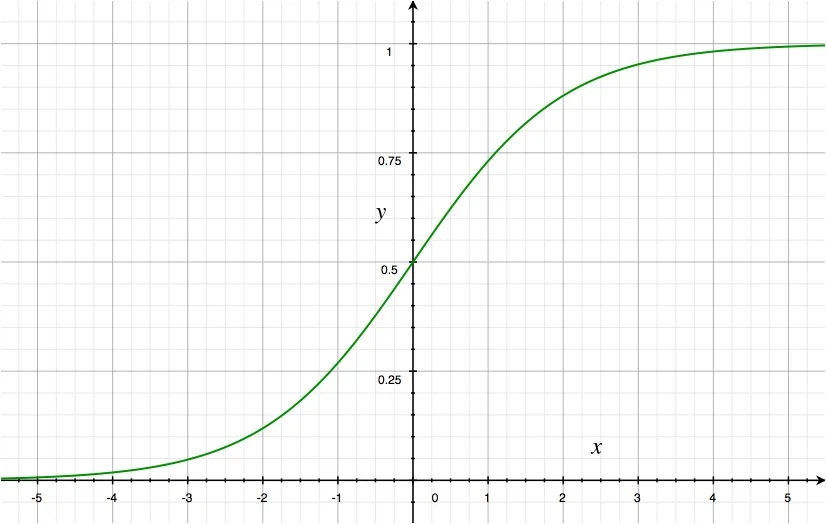
\includegraphics[width=1.0\textwidth]{img/sigmoid.png}
		\caption{Grafico Sigmoide}
	\end{figure}
	
	\[
	\sigma(x) = \frac{1}{1+e^{-x}},\qquad
	\sigma'(x)=\sigma(x)(1-\sigma(x)).
	\]
	\begin{itemize}
		\item \textbf{Pro:} output in \((0,1)\), forma a "S", utile per probabilità (quindi output normalizzato); derivata semplice.
		\item \textbf{Contro:} saturazione per $x\to\pm\infty$ (gradiente $\to0$), quindi soffre di \emph{vanishing gradient} nei layer profondi.
		\item \textbf{Uso tipico:} viene usata nello strato di output per classificazione binaria (in combinazione con binary cross-entropy).
	\end{itemize}
	
	\subsubsection{2. Tangente iperbolica (tanh)}
	
	\begin{figure}[H]
		\centering
		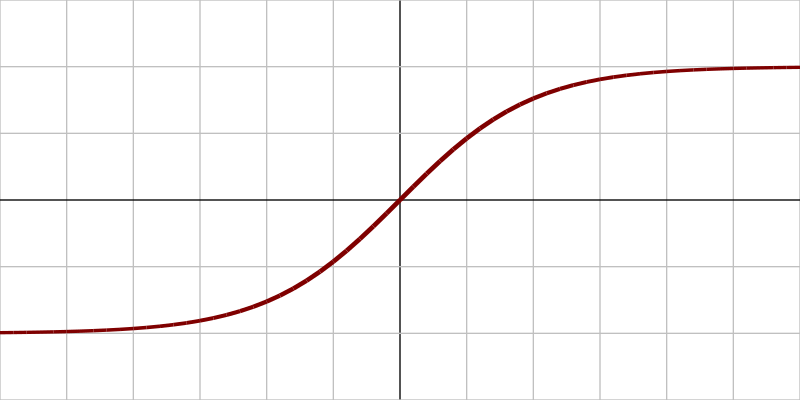
\includegraphics[width=1.0\textwidth]{img/tanh.png}
		\caption{Grafico Tangente iperbolica}
	\end{figure}
	
	\[
	\tanh(x)=\frac{e^x-e^{-x}}{e^x+e^{-x}},\qquad
	\tanh'(x)=1-\tanh^2(x).
	\]
	\begin{itemize}
		\item \textbf{Pro:} output in $(-1,1)$, centrata in $0$, che porta a convergere meglio di sigmoid quando i dati sono normalizzati.
		\item \textbf{Contro:} resta una funzione saturante per valori estremi, quindi può soffrire ancora di vanishing gradient.
		\item \textbf{Uso tipico:} viene usata nei layer nascosti, in reti poco profonde, o quando si desidera un output centrato.
	\end{itemize}
	
	\subsubsection{3. ReLU (Rectified Linear Unit)}
	
	\begin{figure}[H]
		\centering
		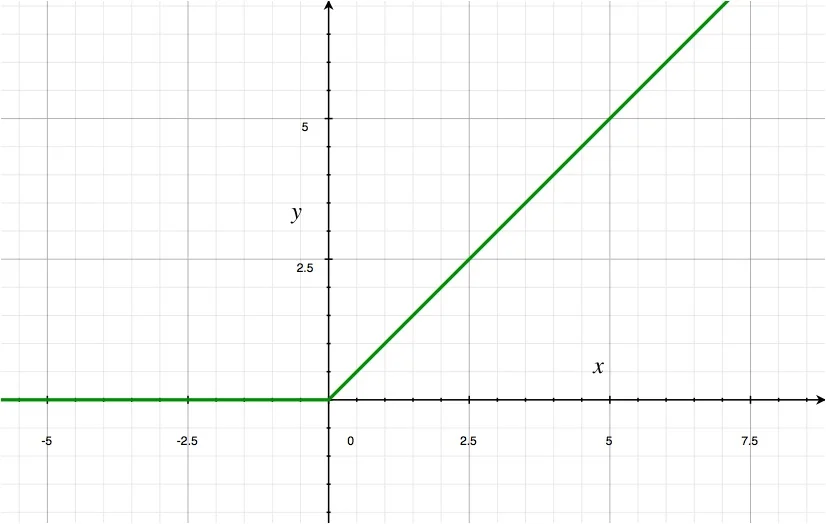
\includegraphics[width=1.0\textwidth]{img/relu.png}
		\caption{Grafico ReLU}
	\end{figure}
	
	\[
	\mathrm{ReLU}(x)=\max(0,x),\qquad
	\mathrm{ReLU}'(x)=\begin{cases}0 & x<0,\\ 1 & x>0,\end{cases}
	\]
	\begin{itemize}
		\item \textbf{Pro:} semplice, computazionalmente efficiente; evita, la maggior parte delle volte, il vanishing gradient sulle porzioni attive; favorisce sparsità delle attivazioni.
		\item \textbf{Contro:} \emph{dying ReLU:} neuroni che restano permanentemente inattivi, se ricevono input negativi grandi; non centrata. Il neurone è morto se, per tutte (o quasi) le istanze del dataset, risulta $x\le0$, allora l’output é sempre uguale a zero. Poiché la derivata di ReLU è zero quando $x<0$, il gradiente, rispetto ai pesi, è zero e quindi quel neurone non riceve più aggiornamenti: resta inattivo per tutto l’allenamento (i pesi non si aggiornano).
		\item \textbf{Uso tipico:} viene usata nei layer nascosti, in quasi tutte le architetture delle reti neurali.
	\end{itemize}
	
	\subsubsection{4. Leaky ReLU (LReLU) / Parametric ReLU (PReLu)}
	
	\begin{figure}[H]
		\centering
		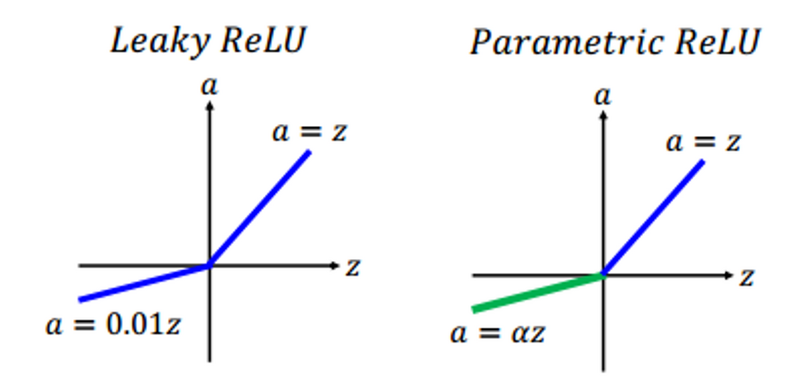
\includegraphics[width=1.0\textwidth]{img/lprelu.png}
		\caption{Grafico LReLU vs PReLU}
	\end{figure}
	
	\[
	\mathrm{LReLU}(x)=\begin{cases}0.01x & x\le0,\\ x & x>0,\end{cases}\qquad
	\mathrm{LReLU}'(x)=\begin{cases}0.01 & x<0,\\ 1 & x>0,\end{cases}\qquad
	\]
	\[
	\mathrm{PReLU}(x)=\begin{cases}\alpha x & x<0,\\ x & x\ge0,\end{cases}\qquad
	\mathrm{PReLU}'(x)=\begin{cases}\alpha & x<0,\\ 1 & x>0,\end{cases}\qquad \alpha\in(0,1)
	\]
	PReLU apprende $\alpha$ durante il training.
	\begin{itemize}
		\item \textbf{Pro:} mantiene un piccolo gradiente per $x<0$, riducendo i \empty{dead neurons}.
		\item \textbf{Contro:} introduce (o apprende) un iperparametro; comportamento non sempre superiore a ReLU.
		\item \textbf{Uso tipico:} dove si vuole evitare il problema del \emph{dying ReLU}, mantenendo semplicità.
	\end{itemize}
	
	\subsubsection{5. ELU (Exponential Linear Unit)}
	
	\begin{figure}[H]
		\centering
		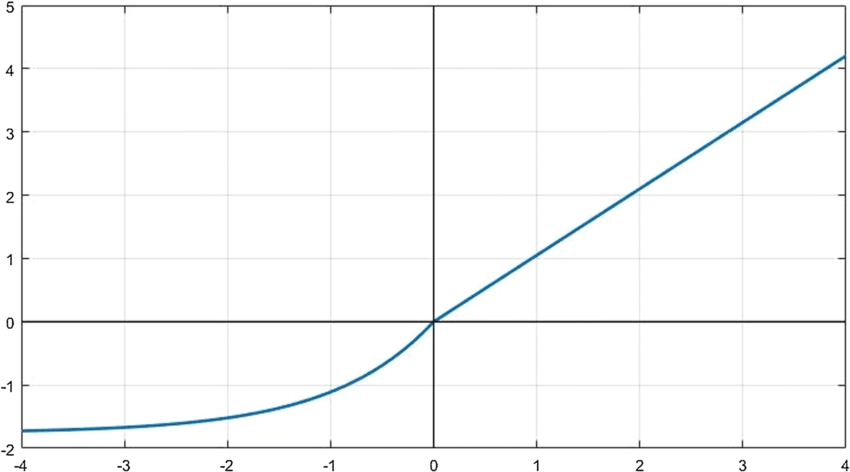
\includegraphics[width=1.0\textwidth]{img/elu.png}
		\caption{Grafico ELU}
	\end{figure}
	
	\[
	\mathrm{ELU}(x)=\begin{cases}x & x\ge0,\\ \alpha(e^x-1) & x<0,\end{cases}\qquad
	\mathrm{ELU}'(x)=\begin{cases}\alpha(e^x) & x<0,\\ 1 & x>0,\end{cases}\qquad \alpha>0
	\]
	\begin{itemize}
		\item \textbf{Pro:} output più centrato, gradiente non nullo per $x<0$, migliore convergenza in alcuni casi.
		\item \textbf{Contro:} leggermente più costosa (esponenziale) e introduce parametro $\alpha$.
	\end{itemize}
	
	\subsubsection{6. Softplus}
	
	\begin{figure}[H]
		\centering
		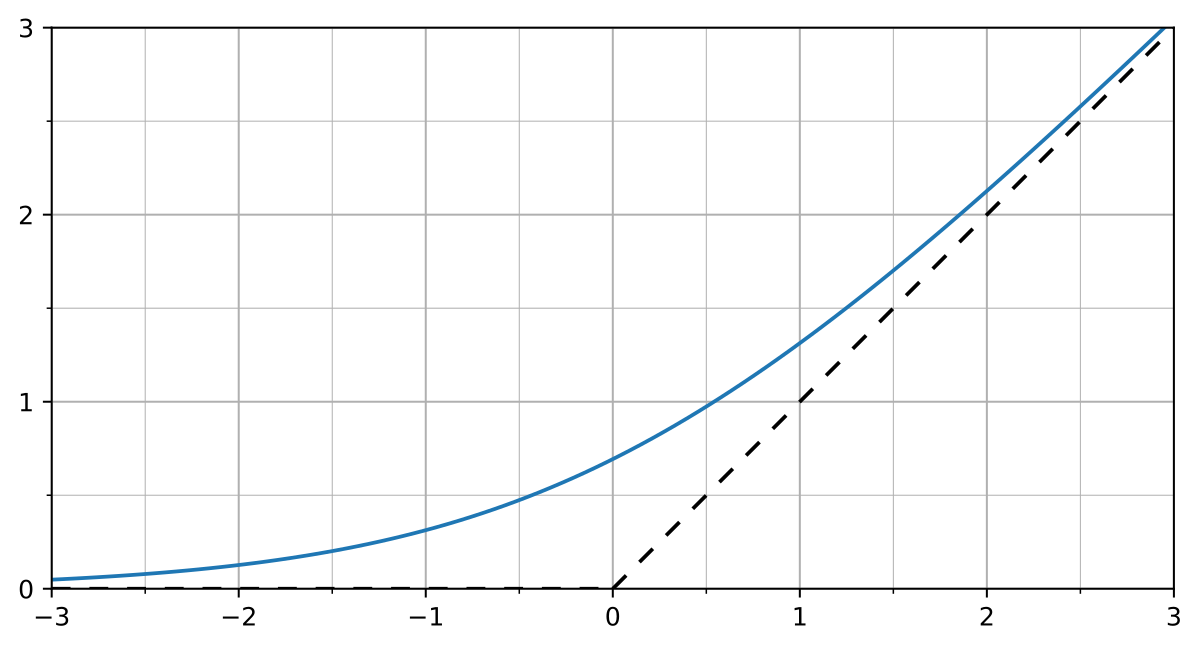
\includegraphics[width=1.0\textwidth]{img/softplus.png}
		\caption{Grafico Softplus}
	\end{figure}
	
	\[
	\mathrm{softplus}(x)=\log(1+e^x),\qquad
	\mathrm{softplus}'(x)=\frac{1}{1+e^{-x}}\qquad
	\]
	\begin{itemize}
		\item \textbf{Pro:} versione smooth e differenziabile di ReLU.
		\item \textbf{Contro:} più costosa e meno sparsa di ReLU.
	\end{itemize}
	
	\subsubsection{7. GELU (Gaussian Error Linear Unit)}
	
	\begin{figure}[H]
		\centering
		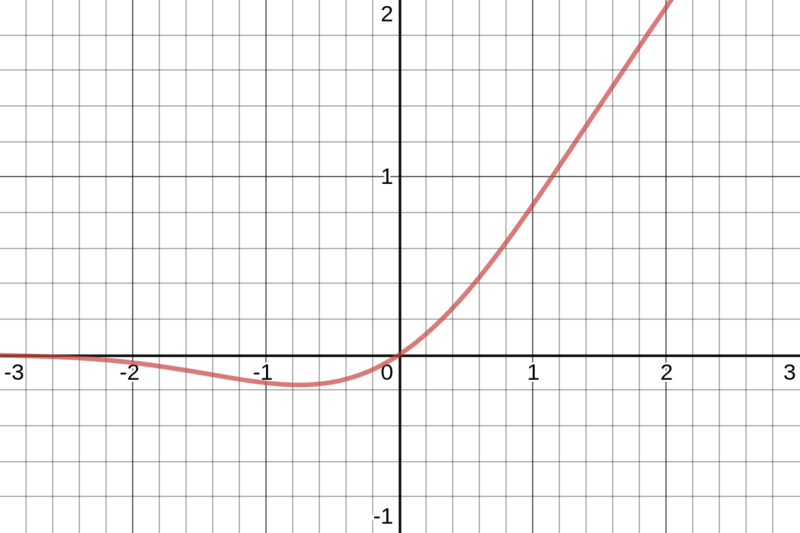
\includegraphics[width=1.0\textwidth]{img/gelu.png}
		\caption{Grafico GELU}
	\end{figure}
	
	\[
	\mathrm{GELU}(x) = x \cdot \Phi(x)
	\]
	dove \(\Phi(x)\) è la funzione di distribuzione cumulativa (CDF) della distribuzione normale standard ed '$\operatorname{erf}$' é la funzione degli errori di Gauss:
	\[
	\Phi(x) = \frac{1}{2} \left[ 1 + \operatorname{erf} \left( \frac{x}{\sqrt{2}} \right) \right] \qquad
	\]
	\[
	\mathrm{GELU}'(x) = \Phi(x) + \frac{1}{2}x\,\phi(x)
	\]
	dove
	\[
	\phi(x) = \frac{1}{\sqrt{2\pi}}\,e^{-x^{2}/2} \qquad
	\]
	\begin{itemize}
		\item \textbf{Pro:} buon comportamento empirico in modelli di linguaggio; più sofisticata della ReLU.
		\item \textbf{Contro:} più costosa da calcolare.
		\item \textbf{Uso tipico:} viene ampiamente utilizzato nelle architetture Transformer; è una funzione di attivazione \empty{soft} che combina linearità e gating stocastico.
	\end{itemize}
	
	\subsubsection{8. Softmax (strato di output per classificazione multi-classe)}
	Per vettore $x\in\mathbb{R}^K$:
	\[
	\mathrm{softmax}(x)_j=\frac{e^{x_j}}{\sum_{k=1}^K e^{x_k}}.
	\]
	\begin{itemize}
		\item \textbf{Uso tipico:} viene utilizzata per trasformare i \emph{logits} in una distribuzione di probabilità, normalmente combinata con la loss di \emph{categorical cross-entropy}.
	\end{itemize}
	
	\subsubsection{Riepilogo}
	\begin{itemize}
		\item \textbf{Hidden layers profondi:} ReLU o varianti (LReLU, PReLU, ELU) sono in genere preferite per ridurre il problema del vanishing gradient e per semplicità computazionale.
		\item \textbf{Reti poco profonde o con output centrato:} tanh può essere utile quando si desidera output centrati.
		\item \textbf{Output:} sigmoide per output binario (con binary cross-entropy); softmax per multi-classe (con categorical cross-entropy); identità (lineare) per regressione.
		\item \textbf{Architetture moderne:} GELU è comune nei Transformers.
		\item \textbf{Sostituti lisci:} softplus può rimpiazzare ReLU quando serve differenziabilità completa.
	\end{itemize}
	La scelta della funzione di attivazione è un trade-off tra proprietà matematiche (saturazione, centering, differenziabilità), efficienza computazionale e comportamento empirico sul problema specifico. Nella maggior parte delle applicazioni moderne la combinazione ReLU (o variante) nei layer nascosti e softmax/sigmoide in output è una scelta robusta, mentre alternative come GELU o ELU possono migliorare le prestazioni in contesti specifici.
	
	\section{Procedura di forward pass}
	
	\subsection{Calcolo delle attivazioni}
	Durante la fase propagazione in avanti (forward pass), i dati attraversano la rete dallo strato di input a quello di output. Ogni neurone calcola prima un ingresso pesato sommandolo con il bias. Dato un neurone $j$ dello strato nascosto o di output, l’attivazione lineare è
	\[
	z_j = \sum_i w_{ji} x_i + b_j,
	\]
	dove $x_i$ sono gli output (o input iniziali), $w_{ji}$ i pesi di connessione, e $b_j$ il bias. In seconda battuta, si applica la funzione di attivazione $\phi$ per ottenere l'uscita del neurone:
	\[
	a_j = \phi(z_j).
	\]
	Ad esempio, con $\phi=\sigma$ (sigmoide), avremmo $a_j=1/(1+e^{-z_j})$. Questo processo viene eseguito strato per strato. Nel primo hidden layer gli ingressi $x_i$ provengono dallo strato di input; nel layer successivo gli ingressi sono le attivazioni $a_j$ del layer precedente, e così via. Ogni layer trasforma in modo non lineare i dati in ingresso, permettendo alla rete di apprendere composizioni funzionali complesse.
	
	\subsection{Propagazione e output}
	Dopo aver calcolato le attivazioni in tutti gli strati intermedi, l'uscita dello strato finale ($\mathbf{a}_{\text{out}}$) costituisce la previsione della rete. Se il problema è di regressione, l'ultima funzione di attivazione può essere identità (o lineare); se è di classificazione binaria, si può usare la sigmoide; se è multi-classe, si usa tipicamente la softmax. Ad esempio, in una classificazione a $K$ classi lo strato di output contiene $K$ neuroni con softmax, e ciascuna uscita $a_k \in (0,1)$ rappresenta la probabilità assegnata alla classe $k$. L'output finale è dunque un vettore di predizioni che dipende dalle scelte di pesi, bias e funzioni di attivazione attraverso la rete. Infine, confrontando $\mathbf{a}_{\text{out}}$ con il valore target (ground truth) del training si calcola una funzione di perdita che misura l'errore di previsione (ad esempio, MSE per regressione o cross-entropy per classificazione). Questa funzione di perdita viene poi utilizzata nell'allenamento per aggiornare i pesi tramite backpropagation.
	
	\section{Algoritmo di backpropagation}
	
	\subsection{Derivazione del gradiente}
	L'algoritmo di backpropagation serve a calcolare come variano i pesi della rete per ridurre l'errore. In termini operativi, si tratta di applicare la \emph{chain rule} per calcolare il gradiente della funzione di perdita $L$ rispetto a ciascun peso $w$. Poiché la rete è una composizione di funzioni (ogni neurone è una funzione di attivazione della sua somma pesata), si propaga l'errore a ritroso layer per layer. Formalmente, a partire dallo strato di output, si calcola la derivata parziale dell'errore rispetto all'attivazione netta di ciascun neurone:
	\[
	\delta_j = \frac{\partial L}{\partial z_j}.
	\]
	Quindi, per il layer precedente si applica la regola della catena: ciascun neurone riceve contributi di errore da tutti i neuroni a cui è connesso nel layer successivo. In pratica, questo permette di ottenere il gradiente di $L$ rispetto a ogni peso:
	\[
	\frac{\partial L}{\partial w_{ji}} = a_i \delta_j,
	\]
	dove $a_i$ è l'uscita del neurone $i$ nel layer precedente e $\delta_j$ è l'``errore locale'' nel neurone $j$. In sostanza, la retropropagazione calcola il gradiente della funzione di perdita rispetto a ogni peso usando la regola della catena per determinare quanto ciascun peso contribuisce all'errore finale. In parole povere, si va all'indietro partendo dall'errore di output e si distribuisce l'errore ai layer precedenti moltiplicando per le derivate delle funzioni di attivazione. Di conseguenza, si ottiene un vettore di gradienti che indica la direzione in cui modificare ciascun peso per diminuire l'errore complessivo.
	
	\subsection{Aggiornamento dei pesi}
	Una volta noti i gradienti parziali $\frac{\partial L}{\partial w}$, i pesi vengono aggiornati solitamente tramite discesa del gradiente (gradient descent). Con un learning rate $\eta$, l'aggiornamento base è dato da:
	\[
	w \leftarrow w - \eta\,\frac{\partial L}{\partial w}.
	\]
	Questo modifica ogni peso nella direzione negativa del gradiente per ridurre la perdita. In termini di formula, per l'esempio di un singolo campione e peso $w_{ji}$:
	\[
	\Delta w_{ji} = -\,\eta\,\frac{\partial L}{\partial w_{ji}} = -\,\eta\,\delta_j\,a_i.
	\]
	Questa è la regola standard di backpropagation con discesa del gradiente. In pratica, si iterano più epoche di allenamento aggiornando i pesi in base a molti esempi, eventualmente con varianti come la discesa del gradiente stocastico (SGD) oppure con algoritmi avanzati (momentum, Adam, ecc.). Tra un passo di forward e il successivo di backward, possono essere applicate tecniche di batching: l'errore può essere aggregato su minibatch di esempi per stabilizzare l'aggiornamento. In ogni caso, il principio fondamentale è che i pesi vengono ``aggiustati'' proporzionalmente al proprio contributo all'errore complessivo, come descritto nelle sezioni precedenti.
	
	\subsection{Tecniche di regolarizzazione}
	Affinché la rete generalizzi bene (non si limiti a riprodurre il rumore dei dati di training), si usano tecniche di regolarizzazione. Due esempi comuni sono:
	
	\begin{itemize}
		\item \textbf{Dropout}: durante l'allenamento, in ciascuna iterazione si disattiva casualmente una parte di neuroni in alcuni layer, impostando le loro attivazioni a zero. In pratica, si costringe la rete a non dipendere eccessivamente da un singolo neurone. Questo riduce l'overfitting in quanto sviluppa più rappresentazioni ridondanti. Ad esempio, con una dropout probability $p$, un neurone viene disattivato con probabilità $p$ e gli altri sono scalati di $1/(1-p)$ per compensazione.
		\item \textbf{Weight decay (regolarizzazione L2)}: si aggiunge al termine di perdita $L$ un fattore $\lambda \|w\|^2$ (con $\lambda>0$), ossia si penalizzano pesi di grandi dimensioni. Questo spinge la rete ad apprendere pesi più piccoli, che tendono a generalizzare meglio riducendo la varianza del modello. In pratica, l'aggiornamento dei pesi incorpora un termine addizionale $-\eta\lambda w$ (decadimento), riducendo la crescita eccessiva di alcuni pesi.
	\end{itemize}
	Entrambe le tecniche (soprattutto il dropout) sono ampiamente usate per evitare che la rete si adatti troppo ai dati di training, per ovviare al problema dell'overfitting. Nel complesso, la regolarizzazione migliora la robustezza del modello, diminuendo l'errore su dati mai visti, migliorando la capacitá di generalizzare del modello.
	
	\section{Vantaggi e limiti}
	
	\subsection{Flessibilità e capacità di generalizzazione}
	Le reti MLP offrono grande flessibilità: grazie alla combinazione di pesi e attivazioni non lineari, possono modellare relazioni complesse e non lineari tra input e output. Come detto, possono apprendere sia compiti di regressione che di classificazione (binarie o multi-classe) e sono in grado di approssimare praticamente qualsiasi funzione continua. Tale capacità di rappresentazione rende le MLP potenti modelli predittivi in molti ambiti (computer vision, NLP, etc.). Inoltre, in presenza di dati adeguati e con l'uso di tecniche di regolarizzazione, le MLP tendono ad avere una buona capacità di generalizzazione, ossia sono in grado di fare previsioni corrette su dati non visti.
	
	\subsection{Problemi di vanishing/exploding gradient}
	Un notevole limite delle MLP (soprattutto se possiedono molti hidden layer) è il problema del vanishing gradient. Poiché, durante la backpropagation, i gradienti vengono moltiplicati per le derivate delle funzioni di attivazione in ogni layer, se queste derivate sono piccole (come nel caso di sigmoidi o tanh, che assumono valori entro $(0,1)$), il prodotto dei gradienti tende a diminuire esponenzialmente con la profondità. Di conseguenza, i pesi nei primi strati (vicini all'input) ricevono gradienti quasi nulli e la rete impara molto lentamente le rappresentazioni nei layer bassi.
	Al contrario, se derivate o pesi sono grandi ($>1$), può manifestarsi un exploding gradient, dove i gradienti crescono esponenzialmente e portano a instabilità numeriche (pesanti oscillazioni o overflow).
	In pratica, questi problemi rendono difficile l'addestramento di reti molto profonde senza accorgimenti: per questo si usano funzioni come le ReLU che hanno derivate più stabili, normalizzazione dei dati, inizializzazione specifiche dei pesi, o architetture speciali per alleviare il fenomeno.
	
	\subsection{Efficienza computazionale}
	Dal punto di vista computazionale, le MLP possono diventare costose da addestrare se il numero di layer o di neuroni è elevato. Ogni propagazione in avanti ed indietro richiede calcoli intensivi (molte moltiplicazioni per matrici di pesi), e su set di dati di grandi dimensioni l'allenamento può richiedere molto tempo e risorse computazionali. Questo si rispecchia nello svantaggio di essere ``computationally expensive''. Il costo cresce con il numero di connessioni del modello. Inoltre, le MLP richiedono un tuning accurato degli iperparametri (learning rate, struttura della rete, regolarizzazione) per ottimizzare performance ed efficienza. In termini pratici, benché le MLP possano essere accelerate su hardware parallelo, allenare reti molto grandi può ancora risultare oneroso e richiede implementazioni attente per gestire efficacemente la complessità.
	
	\chapter{Random Forest}
	
	Il Random Forest è un algoritmo di Machine learning ampiamente utilizzato, noto per la sua robustezza e versatilità sia in problemi di classificazione e regressione. La sua efficacia deriva dalla combinazione di più alberi di decisione "deboli", formando un "ensemble" che supera le prestazioni di un singolo albero, mitigando le debolezze di ciascuno. Questo capitolo esplora i fondamenti, l'architettura e le implicazioni pratiche di Random Forest, iniziando dai suoi blocchi costitutivi: gli alberi di decisione e il paradigma dell'ensemble learning noto come Bagging.
	
	\section{Concetti Fondamentali}
	
	\subsection{Alberi di Decisione: Criteri di Splitting (Gini, Entropia)}
	
	Gli alberi di decisione costituiscono i "learner deboli" fondamentali all'interno di un Random Forest. La loro costruzione implica la divisione iterativa dei dati basata sulle caratteristiche (features) per creare sottoinsiemi sempre più omogenei. La qualità di queste divisioni è misurata da specifici criteri di impurità o guadagno di informazione.
	
	Il Gini impurity (o Gini index) è una misura di non-omogeneità ampiamente utilizzata negli alberi di classificazione, in particolare nell'algoritmo CART (Classification and Regression Trees). Essa quantifica la probabilità che un elemento scelto casualmente da un set venga erroneamente etichettato, se classificato in modo casuale, secondo la distribuzione delle classi nel sottoinsieme. Un valore di 0 indica purezza perfetta, dove tutti gli elementi appartengono alla stessa classe, mentre un valore massimo di 0.5 (per la classificazione binaria) indica la massima impurità, con le classi equamente distribuite. La formula per il Gini impurity è data da:
	
	$$Gini = 1 - \sum_{i=1}^{n} (p_i)^2$$
	
	dove $p_i$ rappresenta la proporzione delle istanze della classe $i$ nel set. Ad esempio, se un nodo contiene 50 campioni, di cui 25 di una classe e 25 di un'altra, l'impurità di Gini sarebbe 0.5, indicando la massima incertezza. Dopo uno split, l'algoritmo seleziona la variabile che produce la maggiore diminuzione dell'impurità di Gini, portando a nodi più puri.
	
	L'Entropia (Entropy) misura il grado di disordine, imprevedibilità o incertezza in un dataset. Un'entropia di 0 indica un set perfettamente puro, mentre un valore di 1 (per la classificazione binaria) indica la massima incertezza. Il Guadagno di informazione (Information Gain) misura la riduzione dell'entropia ottenuta da uno split, indicando quanto "informazione" viene acquisita sulla variabile target. La formula per l'Entropia è:
	
	$$Entropy = - \sum_{i} p_i \log_2(p_i)$$
	
	dove $p_i$ è la probabilità della classe $i$. L'Entropia è tipicamente utilizzata negli algoritmi ID3 e C4.5.
	
	Un confronto tra Gini Impurity ed Entropy rivela differenze importanti. Il Gini impurity ha un intervallo di valori compreso tra $[0, 0.5]$ per la classificazione binaria, mentre l'Entropia ha un intervallo tra $[0, 1]$. Dal punto di vista computazionale, il Gini index è generalmente più efficiente da calcolare rispetto all'entropia, poiché quest'ultima richiede l'uso di logaritmi. Inoltre, il Guadagno di informazione può presentare un bias verso attributi con un gran numero di valori, il che può condurre a un potenziale overfitting, poiché tali attributi tendono a creare molti nodi piccoli e puri. Per mitigare questo bias, è stato introdotto il Gain Ratio (IGR).
	
	La scelta tra Gini e Entropy non è arbitraria, ma implica un compromesso significativo. L'indice di Gini, essendo computazionalmente più veloce, è meno incline a produrre alberi di decisione molto profondi, poiché privilegia split che generano nodi più bilanciati. Al contrario, l'Entropia, sebbene più onerosa dal punto di vista computazionale, tende a generare alberi che massimizzano la riduzione dell'incertezza. Tuttavia, questa sua caratteristica può portare a preferire caratteristiche con molte categorie, aumentando il rischio di overfitting. Per dataset molto grandi o per applicazioni con stringenti requisiti di velocità, il Gini potrebbe essere la scelta preferibile. Per contro, in contesti dove la massima purezza dei nodi è cruciale, l'Entropia (o, più precisamente, il Gain Ratio) potrebbe rivelarsi più efficace, a condizione che il rischio di overfitting venga gestito adeguatamente. Questa decisione fondamentale, a livello del singolo albero, si ripercuote sulla performance e sulla struttura complessiva del Random Forest. Un albero "più debole" ma più rapido, generato con il Gini, può essere efficacemente compensato dall'approccio ensemble, mentre alberi "più forti" ma più lenti, derivanti dall'Entropia, potrebbero non scalare con la stessa efficienza.
	
	\subsection{Ensemble Learning e Bagging}
	
	Random Forest è un esempio di \textbf{Ensemble learning}, una strategia che combina le previsioni di più modelli per ottenere una previsione finale più robusta e accurata rispetto a quanto un singolo modello potrebbe raggiungere.
	
	Il principio alla base è spesso descritto come la "saggezza della folla": un gruppo di learner deboli, che individualmente potrebbero non performare in modo ottimale, a causa di alta varianza o alto bias, può, quando le loro previsioni vengono aggregate, formare un "learner forte" con prestazioni notevolmente migliorate. I metodi ensemble più riconosciuti includono il Bagging ed il Boosting.
	
	Il Bagging è un metodo di Ensemble learning il cui scopo principale è ridurre la varianza all'interno di un dataset "rumoroso", migliorando così la capacità di generalizzazione del modello e mitigando l'overfitting. Il processo di Bagging si articola in tre fasi fondamentali:
	\begin{enumerate}
		\item \textbf{Bootstrapping}: Questa tecnica di ricampionamento genera diversi sottoinsiemi del dataset di training. Il campionamento avviene selezionando istanze in modo casuale con re-immissione, ciò significa che una singola istanza può essere scelta più volte all'interno dello stesso sottoinsieme. Questo processo è cruciale per creare diversità tra i campioni su cui verranno addestrati i modelli individuali.
		\item \textbf{Addestramento Parallelo}: I campioni bootstrap così generati vengono utilizzati per addestrare, in modo indipendente e parallelo, una serie di learner deboli, che nel contesto di Random Forest sono tipicamente alberi di decisione.
		\item \textbf{Aggregazione}: Una volta che i modelli individuali hanno prodotto le loro previsioni, queste vengono combinate. Per i problemi di regressione, si utilizza un processo noto come Soft voting (cioè la media di tutti gli output previsti dai singoli learner), mentre, per i problemi di classificazione, si utilizza l'Hard o Majority voting (cioè viene scelta la classe più votata).
	\end{enumerate}
	
	Il beneficio più significativo è la riduzione della varianza, particolarmente utile con dati ad alta dimensionalità o in presenza di valori mancanti, dove un'alta varianza può rendere il modello più incline all'overfitting. La diversità introdotta nei dati di training per ciascun modello contribuisce a "lisciare" la previsione complessiva, riducendo l'impatto di singoli punti dati rumorosi o outlier nel dataset, rendendo il modello complessivo più robusto e affidabile.
	
	Tuttavia, il Bagging può portare ad una perdita di interpretabilità, rendendo difficile estrarre intuizioni precise a causa del processo di media delle previsioni. È anche computazionalmente costoso, rallentando e diventando più intensivo all'aumentare del numero di iterazioni. Infine, è meno flessibile con algoritmi già stabili o con un alto bias, poiché i benefici, in termini di riduzione della varianza, sono meno visibili.
	
	Il Bagging non è semplicemente un metodo per combinare modelli, ma agisce come una forma intrinseca di regolarizzazione. Addestrando modelli su sottoinsiemi diversi del dataset, attraverso il campionamento di tipo bootstrap, si garantisce che ogni modello acquisisca una prospettiva leggermente differente del problema. Quando le previsioni di questi modelli, sebbene diversi, sono aggregate, gli errori casuali e la varianza intrinseca di un singolo modello tendono a compensarsi reciprocamente. Ciò porta a una previsione finale che è più stabile e meno sensibile al rumore oppure agli outlier. Questo meccanismo è la ragione fondamentale per cui il Bagging è così efficace nel ridurre l'overfitting, specialmente per learner ad alta varianza, come gli alberi di decisione profondi. Questa capacità di ridurre la varianza senza introdurre un bias significativo è ciò che rende il Bagging una base così potente per algoritmi come Random Forest, che altrimenti sarebbero molto inclini all'overfitting. È una dimostrazione del principio che la "diversità" all'interno di un ensemble conduce a una maggiore robustezza del modello complessivo.
	
	\section{Architettura e Costruzione}
	
	Random Forest estende il concetto di Bagging introducendo un ulteriore livello di casualità, rendendo l'ensemble di alberi ancora più robusto e meno propenso all'overfitting.
	
	\subsection{Campionamento Bootstrap e Casualità delle Feature}
	
	La costruzione di un Random Forest si basa su due fonti principali di casualità, essenziali per garantire che gli alberi individuali siano il più possibile non correlati tra loro.
	
	La prima fonte di casualità è il campionamento di tipo bootstrap (Bagging). Per ogni albero che fa parte della foresta, viene estratto un campione casuale di dati dal set di training originale con re-immissione. Questo sottoinsieme di dati è noto come "bootstrap sample". Una caratteristica importante di questo processo è che circa un terzo dei dati originali non viene selezionato per un dato bootstrap sample; questi dati non utilizzati sono chiamati campioni "out-of-bag" (OOB) e possono essere impiegati per la validazione interna del modello, eliminando la necessità di un set di convalida separato. Questo tipo di campionamento assicura che ogni albero sia addestrato su un sottoinsieme leggermente diverso dei dati originali, promuovendo una diversità fondamentale tra gli alberi.
	
	La seconda fonte di casualità è legata alle features, nota come feature bagging o random subspace method. Ad ogni split dei nodi, all'interno di un albero di decisione, Random Forest non considera tutte le feature disponibili, ma seleziona solo un sottoinsieme casuale di esse. Questa è una differenza cruciale rispetto agli alberi di decisione standard, che valuterebbero tutte le feature possibili per trovare lo split migliore. L'introduzione di questa casualità nella selezione delle feature aggiunge ulteriore diversità al dataset per ogni albero e riduce significativamente la correlazione tra gli alberi di decisione individuali, un fattore chiave per la robustezza del Random Forest.
	
	La casualità introdotta sia nel campionamento dei dati sia nella selezione delle feature per ogni split non è ridondante, ma complementare e strategica. Il bagging riduce la varianza generale del modello assicurando che ogni albero acquisisca una prospettiva leggermente diversa del dataset complessivo. La casualità delle feature, d'altra parte, previene che caratteristiche particolarmente forti o dominanti influenzino la costruzione di tutti gli alberi. Se una singola caratteristica fosse sempre scelta come il miglior punto di split, tutti gli alberi all'interno della foresta risulterebbero molto simili e altamente correlati, rendendo inutili i benefici derivanti dall'approccio Ensemble. Introducendo la casualità nella selezione delle feature, si forza ogni albero ad esplorare diverse combinazioni di caratteristiche, riducendo ulteriormente la loro correlazione e, di conseguenza, la varianza dell'intero Ensemble. Questa doppia "randomizzazione" è il cuore della robustezza del Random Forest contro l'overfitting. Essa non si limita a ridurre la varianza, ma lo fa in modo più efficace rispetto al solo bagging, creando un ensemble di alberi veramente "diversi" che, quando aggregati, producono una previsione più stabile e generalizzabile.
	
	\subsection{Aggregazione delle Predizioni}
	
	Una volta che tutti gli alberi di decisione sono stati costruiti e addestrati sui rispettivi sottoinsiemi di dati e feature, le loro previsioni vengono combinate per ottenere il risultato finale del Random Forest. Il metodo di aggregazione dipende dalla natura del problema:
	\begin{itemize}
		\item \textbf{Per Problemi di Regressione}: Quando il Random Forest è utilizzato per compiti di regressione, le previsioni numeriche generate da ciascun albero individuale vengono semplicemente mediate. Il valore medio di tutte le previsioni degli alberi costituisce la previsione finale del modello. Questo processo è talvolta chiamato \textbf{Soft voting}.
		\item \textbf{Per Problemi di Classificazione}: Per i compiti di classificazione, la classe finale viene determinata attraverso un processo di voto di maggioranza. Ogni albero nella foresta produce una previsione e la classe che riceve il maggior numero di "voti" (cioè, la più scelta) tra tutti gli alberi viene accettata come previsione finale del Random Forest. Questo è noto come \textbf{Hard voting} o \textbf{Majority voting}.
	\end{itemize}
	
	L'aggregazione delle previsioni, sia essa tramite media o voto di maggioranza, rappresenta il passo finale che trasforma un insieme di learner deboli in uno forte. Sebbene gli alberi di decisione individuali possano presentare un'alta varianza, ovvero una tendenza a overfittare i dati di training, l'atto di mediare o votare le loro previsioni tende a "lisciare" le anomalie e le specificità di ogni singolo albero. Questo processo riduce efficacemente la varianza complessiva del modello ensemble senza introdurre un bias significativo, a condizione che gli alberi siano sufficientemente "deboli" ma non eccessivamente correlati tra loro. Questo meccanismo di aggregazione è ciò che consente al Random Forest di raggiungere un'elevata accuratezza mantenendo al contempo una solida capacità di generalizzazione. È un esempio pratico dell'applicazione del principio della "saggezza della folla" nel Machine learning, dove la combinazione di molteplici opinioni individuali, seppur imperfette, conduce ad un risultato complessivo superiore.
	
	\section{Vantaggi e Svantaggi}
	
	I vantaggi del Random Forest sono numerosi e spiegano la sua ampia adozione:
	\begin{itemize}
		\item \textbf{Alta Accuratezza}: Spesso supera altri algoritmi in termini di accuratezza predittiva per problemi sia di classificazione che di regressione.
		\item \textbf{Riduzione dell'Overfitting}: È intrinsecamente meno propenso all'overfitting rispetto a un singolo albero di decisione. Questo è dovuto alla sua natura ensemble, che aggrega le previsioni di molti alberi diversi, e all'introduzione di casualità sia nel campionamento dei dati che nella selezione delle feature.
		\item \textbf{Robustezza agli Outlier e ai Dati Rumorosi}: Il modello è meno suscettibile all'influenza degli outlier, poiché le previsioni vengono mediate su più alberi, diluendo l'impatto di singole osservazioni estreme. Per i dati rumorosi, l'approccio del bagging è particolarmente promettente.
		\item \textbf{Gestione dei Valori Mancanti}: Random Forest può gestire efficacemente i valori mancanti nel dataset senza la necessità di tecniche di imputazione complesse, rendendo il pre-processing dei dati più semplice.
		\item \textbf{Gestione Dati Sbilanciati}: Ha la capacità di gestire dataset in cui le classi sono sbilanciate, sebbene la sua performance possa variare in condizioni di forte sbilanciamento rispetto ad altri algoritmi.
		\item \textbf{Facilità di Determinazione dell'Importanza delle Feature}: L'algoritmo rende relativamente semplice valutare il contributo di ciascuna variabile al modello, fornendo una misura dell'importanza delle feature.
		\item \textbf{Versatilità}: È applicabile sia a problemi di regressione che di classificazione, il che lo rende uno strumento flessibile per diverse tipologie di analisi.
		\item \textbf{Parallelizzabile}: I singoli alberi all'interno del Random Forest possono essere addestrati in parallelo. Questa caratteristica contribuisce significativamente alla sua velocità di addestramento, specialmente quando si lavora con dataset di grandi dimensioni e hardware multi-core.
	\end{itemize}
	
	Nonostante i suoi numerosi pregi, il Random Forest presenta anche alcuni svantaggi:
	\begin{itemize}
		\item \textbf{Costo Computazionale e Tempo di Addestramento}: L'addestramento di un Random Forest può essere lento, in particolare con un numero molto elevato di alberi o su dataset di grandi dimensioni, poiché la costruzione di ogni albero è un'operazione computazionalmente intensiva.
		\item \textbf{Requisiti di Risorse}: Poiché elabora dataset potenzialmente grandi e costruisce molti alberi, richiede più risorse di memoria per archiviare i dati rispetto a un singolo albero.
		\item \textbf{Complessità e Perdita di Interpretability (rispetto a un singolo albero)}: Sebbene un singolo albero di decisione sia intrinsecamente interpretabile, la previsione di una "foresta" di centinaia o migliaia di alberi diventa molto più difficile da interpretare a livello globale. Il modello complessivo può essere visto come una "scatola nera".
		\item \textbf{Mancanza di Regolarizzazione Esplicita}: A differenza di altri algoritmi ensemble, Random Forest non include tecniche di regolarizzazione dirette, come la penalizzazione di modelli complessi (regolarizzazione L1 o L2). Si affida principalmente alla sua natura ensemble e all'introduzione di casualità per prevenire l'overfitting.
	\end{itemize}
	
	Il Random Forest è spesso elogiato per la sua capacità di fornire punteggi di importanza delle feature, un aspetto che lo rende più interpretabile rispetto a molti modelli complessi. Tuttavia, a livello di modello globale, la sua natura ensemble, composta da centinaia o migliaia di alberi, lo rende una "scatola nera". Non è possibile tracciare un singolo percorso decisionale come si farebbe con un albero singolo. Questo crea un paradosso: si può comprendere quali feature sono importanti, ma non come il modello giunge a una decisione specifica per un dato input. Questo compromesso è cruciale nella scelta di un modello per applicazioni reali. In settori come la finanza o la medicina, dove la spiegabilità delle decisioni è fondamentale, la perdita di interpretabilità a livello di modello può rappresentare un ostacolo, nonostante la chiarezza sull'importanza delle feature. Questa limitazione spinge all'utilizzo di tecniche di spiegabilità post-hoc, anche per il Random Forest, sebbene siano più comunemente associate alle reti neurali.
	
	\chapter{eXtreme Gradient Boosting (XGBoost)}
	
	XGBoost è un'implementazione avanzata e altamente ottimizzata del framework di Gradient Boosting, che ha guadagnato enorme popolarità per la sua velocità e precisione in una vasta gamma di problemi di Machine learning. Questo capitolo approfondirà i principi fondamentali del boosting, le innovazioni che distinguono XGBoost dai metodi tradizionali di Gradient Boosting, i suoi parametri chiave e le sue prestazioni.
	
	\section{Introduzione al Gradient boosting}
	
	Il Gradient boosting è una potente tecnica di Ensemble learning che costruisce un modello predittivo forte combinando iterativamente i risultati di numerosi "learner deboli". A differenza del Bagging, che addestra i modelli in parallelo, il Boosting adotta un approccio sequenziale, dove ogni nuovo modello cerca di correggere gli errori commessi dai modelli precedenti.
	
	\subsection{Principi iterativi e Weak learners}
	
	Il gradient boosting si fonda sull'idea di migliorare progressivamente un modello addestrando nuovi learner per correggere gli errori commessi dai precedenti. Questo processo è intrinsecamente iterativo e sequenziale. A differenza del Bagging, dove i learner sono addestrati in modo parallelo ed indipendente, il gradient boosting costruisce un modello additivo passo dopo passo. Ogni nuovo "albero" (che funge da learner debole) viene costruito specificamente per ridurre gli errori, o più precisamente gli "pseudo-residui", generati dalle previsioni degli alberi addestrati nelle iterazioni precedenti.
	I "learner deboli", in questo caso, sono modelli che, se utilizzati singolarmente, classificano o predicono i dati in modo scarso, talvolta non meglio di un'ipotesi casuale, e presentano un alto tasso di errore. Nel framework del gradient boosting, questi learner deboli sono tipicamente alberi di decisione semplici. Possono essere molto poco profondi, a volte ridotti ad un singolo split, in tal caso sono noti come "decision stumps". L'obiettivo generale del gradient boosting è minimizzare una funzione di perdita predefinita, aggiungendo iterativamente funzioni (i learner deboli) che puntano nella direzione del gradiente negativo della funzione di perdita stessa.
	Mentre il Bagging mira a ridurre la varianza addestrando modelli indipendenti e poi mediandone i risultati, il Boosting si concentra sulla riduzione del bias del modello. Addestrando sequenzialmente nuovi learner per correggere gli errori dei precedenti, il modello impara a concentrarsi sulle istanze più difficili da classificare o predire. Questo processo iterativo consente al modello di adattarsi in modo più efficace alle relazioni complesse presenti nei dati, riducendo il bias complessivo e portando spesso a una maggiore accuratezza predittiva. Questa differenza fondamentale nell'approccio, ovvero la riduzione della varianza contro la riduzione del bias, spiega perché il Bagging ed il Boosting eccellono in contesti diversi e perché algoritmi come Random Forest e XGBoost possiedono caratteristiche di performance distinte.
	
	\subsection{Funzione di perdita e Discesa del gradiente}
	
	Il processo di apprendimento nel gradient boosting è formalizzato come un algoritmo di discesa del gradiente nello spazio delle funzioni, dove l'obiettivo è trovare la funzione che minimizza la funzione di perdita, che quantifica quanto bene il modello sta eseguendo le previsioni sui dati forniti. La scelta della funzione di errore dipende dalla natura del problema: ad esempio, per problemi di regressione si potrebbe usare l'errore quadratico medio (MSE), mentre per problemi di classificazione si potrebbe usare la log-loss. L'algoritmo di gradient boosting mira a minimizzare questa funzione di perdita.
	In ogni iterazione, il modello calcola i cosiddetti "pseudo-residui", che non sono i residui tradizionali (differenza tra valore osservato e previsto), ma piuttosto i gradienti negativi della funzione di perdita rispetto alle previsioni attuali del modello. Il nuovo learner debole (tipicamente un albero di decisione) viene quindi addestrato per predire questi pseudo-residui, imparando così a correggere gli errori del modello ensemble cumulativo.
	Il processo di aggiunta di nuovi alberi può essere interpretato come un passo nella direzione del gradiente negativo della funzione di perdita nello spazio delle funzioni. Un'innovazione significativa in XGBoost rispetto al gradient boosting tradizionale è l'utilizzo di un'approssimazione di Taylor del secondo ordine nella funzione di perdita. Questo approccio collega il processo di ottimizzazione di XGBoost al metodo Newton-Raphson, che è più robusto e può portare a una convergenza più rapida rispetto alla discesa del gradiente del primo ordine.
	L'utilizzo di un'approssimazione di Taylor del secondo ordine nella funzione di perdita distingue XGBoost dal gradient boosting tradizionale, che si basa sul gradiente del primo ordine. Ciò implica che XGBoost considera, non solo la direzione di discesa più ripida (data dal gradiente), ma anche la curvatura della funzione di perdita (data dall'hessiana). Ciò consente al modello di compiere passi più informati e potenzialmente più ampi verso il minimo della funzione di perdita, portando a una convergenza più rapida e stabile. Di conseguenza, XGBoost risulta meno sensibile a problemi come i minimi locali rispetto agli algoritmi che utilizzano esclusivamente il gradiente del primo ordine. Questa modifica è uno dei motivi principali della superiorità prestazionale di XGBoost in numerose competizioni di machine learning ed in svariate applicazioni reali. Dimostra come un'implementazione più avanzata dei principi fondamentali possa tradursi in miglioramenti significativi in termini di prestazioni ed efficienza del modello.
	
	\section{Miglioramenti di XGBoost rispetto al Gradient boosting tradizionale}
	
	XGBoost è riconosciuto come un'evoluzione del gradient boosting, grazie all'integrazione di una serie di ottimizzazioni e tecniche di regolarizzazione che ne migliorano significativamente prestazioni, velocità e robustezza.
	
	\subsection{Regolarizzazione e Tree pruning}
	
	XGBoost si distingue per l'integrazione di meccanismi di regolarizzazione configurabili, che sono cruciali per prevenire l'overfitting e migliorare la sua capacitá di generalizzare.
	Il modello incorpora termini di regolarizzazione L1 (Lasso) e L2 (Ridge), direttamente nella sua funzione obiettivo. Questi termini penalizzano la complessità del modello ed i pesi di grandi dimensioni, contribuendo a mitigare l'overfitting. In particolare, la regolarizzazione L1 incoraggia la sparsità, spingendo i pesi meno importanti verso lo zero, mentre la regolarizzazione L2 incoraggia pesi più piccoli e distribuiti. \\
	Una componente fondamentale della regolarizzazione nel gradient boosting è il "learning rate" (o shrinkage). Questo parametro scala il contributo di ogni nuovo albero aggiunto al modello. Inoltre, é stato dimostrato che l'uso di learning rate piccoli (ad esempio, 0.01 o 0.1) migliori di molto la capacità di generalizzazione del modello, sebbene ciò comporti un aumento del numero di iterazioni e, di conseguenza, del tempo di calcolo. \\
	XGBoost implementa anche tecniche avanzate di tree pruning. A differenza di alcuni algoritmi che costruiscono alberi fino alla massima profondità, XGBoost non lo fa. La potatura avviene in base ad un "guadagno" del nodo. L'iperparametro "gamma" specifica la riduzione minima della funzione di errore richiesta per effettuare un'ulteriore partizione su un nodo foglia. Un valore più grande di questo rende l'algoritmo più conservativo, limitando la crescita dell'albero ed aiutando a prevenire l'overfitting. \\
	Un altro parametro cruciale per la regolarizzazione è la "somma minima dei pesi delle istanze". Questo definisce la somma minima del peso delle istanze (basata sull'hessiana della funzione di perdita) necessaria in un nodo figlio per consentire un ulteriore split. Se esso si traduce in un nodo foglia con un peso inferiore all'iperparametro, la partizione viene annullata, mentre un valore più grande, rende l'algoritmo più conservativo, riducendo la complessità degli alberi individuali. \\
	A differenza di Random Forest, che si affida principalmente alla sua natura ensemble per ridurre l'overfitting, XGBoost integra meccanismi di regolarizzazione configurabili. Questa capacità di adeguare il modello per controllare la sua complessità e la sua tendenza all'overfitting è un vantaggio significativo. Permette ai data scientist di bilanciare in modo più preciso bias e varianza, spesso portando a prestazioni superiori su dati complessi.
	
	\subsection{Gestione dei valori mancanti}
	
	XGBoost si distingue per il suo approccio sofisticato e trasparente alla gestione dei valori mancanti, una caratteristica che lo rende particolarmente robusto ed efficiente in contesti reali dove i dataset sono spesso incompleti.
	Il modello implementa un algoritmo, consapevole della sparsità, che gestisce i valori mancanti in modo flessibile. Durante la costruzione degli alberi di decisione, quando viene incontrato un valore mancante per una determinata feature, XGBoost non si limita a ignorare o richiedere una rimozione preliminare di essa. Invece, l'algoritmo è in grado di prendere una decisione su quale ramo del nodo (sinistra o destra) il dato debba prendere, basandosi sui dati disponibili. Internamente, durante la fase di training, XGBoost apprende la direzione ottimale da seguire per le istanze con valori mancanti, trattando la "mancanza" del dato come una caratteristica informativa a sé stante.
	Molti algoritmi richiedono una rimozione esplicita dei valori mancanti, un processo che può introdurre bias o rumore nel dataset ed aumentare la complessità del pre-processing. La capacità di XGBoost di gestire i valori mancanti internamente, imparando la direzione ottimale per gli split, rappresenta un vantaggio significativo. Questo non solo semplifica la pipeline di preparazione dei dati, ma può anche portare a modelli più robusti, poiché il modello apprende direttamente dalla "mancanza" dell'informazione, piuttosto che da un'eliminazione potenzialmente errata o arbitraria. Questa funzionalità rende XGBoost particolarmente efficiente e pratico per dataset reali, che spesso contengono valori mancanti, riducendo la necessità di avere una fase di Data pre-processing complessa, migliorando così l'affidabilità del modello in scenari del mondo reale.
	
	\subsection{Ottimizzazioni (Parallelismo, Cache-Awareness)}
	
	Una delle ottimizzazioni chiave di XGBoost è il parallelismo. Sebbene il gradient boosting sia intrinsecamente sequenziale nella costruzione degli alberi (ogni albero corregge gli errori del precedente), XGBoost introduce il parallelismo, nella costruzione dei singoli alberi, in particolare sui livelli dell'albero o di split. Questo significa che, anziché costruire gli alberi in modo strettamente sequenziale, XGBoost può scansionare i valori del gradiente ed utilizzare somme parziali per valutare la qualità degli split in parallelo. Il sistema sfrutta tutti i core della CPU disponibili su una singola macchina e può operare in modalità distribuita, massimizzando l'utilizzo della potenza di calcolo. Questo parallelismo su larga scala accelera significativamente il processo di addestramento. \\
	Un'altra ottimizzazione interessante è il cache-awareness. XGBoost è progettato per utilizzare in modo intelligente la cache della CPU per accelerare l'accesso ai dati. Durante l'addestramento, memorizza nella cache i calcoli intermedi e le statistiche importanti, evitando così di ricalcolare gli stessi valori ripetutamente. Questo riduce i ritardi nel recupero dei dati tra la CPU e memoria principale, portando ad un'elaborazione e previsioni molto più veloci. \\
	Infine, XGBoost beneficia della GPU acceleration, che velocizza significativamente l'addestramento del modello e contribuisce a migliorare l'accuratezza delle previsioni. L'algoritmo sfrutta il calcolo parallelo per eseguire operazioni veloci, come Prefix sum e Parallel radix sort, per ripartizionare i dati e costruire gli alberi un livello alla volta, elaborando l'intero dataset contemporaneamente sulla GPU. \\
	
	\section{Parametri chiave e Tuning}
	
	XGBoost offre un'ampia e dettagliata lista di iperparametri che possono essere ottimizzati per personalizzare il comportamento del modello e massimizzare le sue prestazioni. Questa flessibilità, sebbene potente, richiede una comprensione approfondita ed un'attenta strategia di tuning.
	I parametri per il Tree Booster controllano la costruzione dei singoli alberi all'interno dell'Ensemble:
	\begin{itemize}
		\item \texttt{learning\_rate} (o \texttt{eta}): Questo è il tasso di apprendimento, un parametro cruciale che controlla la dimensione del passo di shrinkage per prevenire l'overfitting. Valori più piccoli di \texttt{eta} rendono il processo di boosting più conservativo, riducendo il rischio di overfitting ma richiedendo più iterazioni. Il suo intervallo è $(0, 1]$.
		\item \texttt{max\_depth}: Definisce la profondità massima di un albero. Aumentare questo valore rende il modello più complesso e potenzialmente più incline all'overfitting. Un valore di $0$ indica nessuna limitazione di profondità, ma ciò può portare a un elevato consumo di memoria. L'intervallo è $[0, \infty]$.
		\item \texttt{min\_child\_weight}: Specifica la somma minima del peso delle istanze (basata sull'hessiana) necessaria in un nodo figlio per consentire un ulteriore split. Un valore più grande rende l'algoritmo più conservativo, limitando la crescita dell'albero. L'intervallo è $[0, \infty]$.
		\item \texttt{subsample}: Rappresenta la frazione di osservazioni (istanze) campionate casualmente per la costruzione di ogni albero. Questo campionamento avviene una volta per ogni iterazione di boosting ed aiuta a prevenire l'overfitting. L'intervallo è $(0, 1]$.
		\item \texttt{colsample\_bytree}: Indica la frazione di features campionate casualmente per la costruzione di ogni albero. Questo parametro contribuisce anch'esso a prevenire l'overfitting introducendo casualità nella selezione delle caratteristiche. L'intervallo è $(0, 1]$.
		\item \texttt{lambda} (o \texttt{reg\_lambda}): È il termine di regolarizzazione L2 sui pesi. Aumentare questo valore rende il modello più conservativo, penalizzando i pesi grandi. L'intervallo è $[0, \infty)$.
		\item \texttt{alpha} (o \texttt{reg\_alpha}): È il termine di regolarizzazione L1 sui pesi. Un valore più grande rende il modello più conservativo e incoraggia la sparsità, spingendo i pesi meno importanti verso lo zero. L'intervallo è $[0, \infty]$.
	\end{itemize}
	I parametri del problema di apprendimento definiscono l'obiettivo di ottimizzazione e le metriche di valutazione:
	\begin{itemize}
		\item \texttt{objective}: Definisce la funzione di perdita che il modello mira a minimizzare. Esempi comuni includono \texttt{reg:squarederror} per problemi di regressione, \texttt{binary:logistic} per classificazione binaria e \texttt{multi:softprob} (che produce probabilità) per classificazione multiclasse.
		\item \texttt{eval\_metric}: Specifica la metrica di valutazione da monitorare durante l'addestramento. È possibile specificare più metriche. Esempi includono \texttt{rmse} (Root Mean Square Error) per la regressione, \texttt{logloss} (Negative Log-likelihood), \texttt{error} (tasso di errore di classificazione), \texttt{merror} (tasso di errore multiclasse), \texttt{aucroc} (Area Under the Curve ROC) e \texttt{aucpr} (Area Under the Precision-Recall Curve).
	\end{itemize}
	Per l'ottimizzazione dei parametri, sono essenziali diverse tecniche:
	\begin{itemize}
		\item \textbf{Hyperparameter Tuning}: Tecniche come Grid Search, Random Search, Bayesian optimization o Genetic algorithm sono cruciali per esplorare lo spazio degli iperparametri e trovare la combinazione ottimale che massimizza le prestazioni del modello.
		\item \textbf{Early Stopping}: Questa è una tecnica fondamentale per prevenire l'overfitting. Consiste nell'interrompere l'addestramento del modello se la metrica di validazione su un set di dati separato non migliora per un certo numero di round consecutivi. Ciò impedisce al modello di continuare ad apprendere il rumore nei dati di training una volta che le sue prestazioni di generalizzazione iniziano a peggiorare.
	\end{itemize}
	L'ampia gamma di iperparametri in XGBoost offre un controllo granulare sul comportamento del modello, ma al contempo introduce una significativa complessità nel processo di tuning. A differenza di Random Forest, che tende ad avere meno parametri da ottimizzare, XGBoost richiede una comprensione più approfondita e una sperimentazione più estesa per raggiungere le sue prestazioni ottimali. Questo implica che, sebbene XGBoost possa teoricamente superare Random Forest in termini di accuratezza, raggiungere tale superiorità richiede un investimento maggiore in termini di tempo e risorse per il tuning. Questa osservazione è fondamentale per la scelta del modello in base alle risorse ed agli obiettivi del progetto.
	
	\section{Vantaggi}
	
	\begin{itemize}
		\item \textbf{Accuratezza superiore}: XGBoost raggiunge frequentemente un'accuratezza predittiva maggiore rispetto a molti altri algoritmi, in particolare su dati strutturati/tabulari ed in situazioni complesse. È spesso l'algoritmo di scelta nelle competizioni di machine learning, come quelle su Kaggle, dove l'obiettivo è la massima precisione possibile.
		\item \textbf{Robustezza all'overfitting}: grazie alle sue varie tecniche di regolarizzazione integrate, XGBoost è molto robusto contro l'overfitting. Questo controllo granulare sulla complessità del modello è un fattore chiave della sua capacità di generalizzazione.
		\item \textbf{Gestione efficiente di grandi dataset}: è stato progettato per scalabilità ed efficienza, gestendo efficacemente dati di grandi dimensioni, dati sparsi e valori mancanti. La sua architettura ottimizzata consente di elaborare grandi quantità di dati che sarebbero impossibili da gestire per altri algoritmi.
		\item \textbf{Velocità di addestramento}: nonostante la sua natura sequenziale, XGBoost è altamente ottimizzato per la velocità. Può essere più veloce di Random Forest nell'addestramento, specialmente quando si sfruttano le sue capacità di parallelismo e l'accelerazione GPU, oltre al supporto per sistemi distribuiti.
		\item \textbf{Flessibilità e Personalizzazione}: Offre un'ampia gamma di iperparametri che consentono un fine-tuning profondo del modello, adattandolo alle specifiche esigenze del problema e dataset.
		\item \textbf{Gestione dati sbilanciati}: è particolarmente efficace nella gestione di dataset con classi sbilanciate, fornendo parametri specifici come \texttt{scale\_pos\_weight} per bilanciare i pesi delle classi e migliorare le prestazioni sulla classe minoritaria.
	\end{itemize}
	
	\section{Svantaggi}
	
	\begin{itemize}
		\item \textbf{Processo di addestramento sequenziale}: nonostante le ottimizzazioni per il parallelismo interno, la sua natura di boosting sequenziale (dove ogni albero dipende dal precedente) può renderlo intrinsecamente più lento di Random Forest nella costruzione degli alberi completi, a meno che non si sfruttino appieno le sue capacità di parallelismo e le accelerazioni hardware.
		\item \textbf{Complessità e Tuning}: è un algoritmo più complesso da comprendere ed implementare rispetto al Random Forest. La sua vasta gamma di iperparametri richiede una maggiore conoscenza ed esperienza per un fine-tuning efficace, rendendo il processo più dispendioso in termini di tempo e risorse.
		\item \textbf{Meno interpretabile di Random Forest (a volte)}: sebbene fornisca l'importanza delle feature, la complessità dell'ensemble di alberi sequenziali può rendere le sue decisioni specifiche più difficili da interpretare rispetto ad un Random Forest, dove spesso si richiedono strumenti aggiuntivi per la spiegabilità.
		\item \textbf{Consumo di memoria}: può consumare una notevole quantità di memoria, specialmente quando si addestrano alberi molto profondi, il che può essere una limitazione per dataset estremamente grandi su hardware con risorse limitate.
	\end{itemize}
	
	\chapter{Convolutional Neural Networks (CNN)}
	
	\section{Principi fondamentali delle CNN}
	
	\subsection{Convoluzione: kernel, stride, padding}
	Le Convolutional Neural Networks (CNN) rappresentano una classe specializzata di reti neurali progettate per elaborare dati con struttura a griglia, come le immagini. L'operazione fondamentale su cui si basano è la convoluzione, una trasformazione matematica che applica filtri (kernel) all'input per estrarre caratteristiche locali.
	
	Un kernel (o filtro) è una matrice di piccole dimensioni, tipicamente 3$\times$3, 5$\times$5 o 7$\times$7, contenente pesi apprendibili che vengono moltiplicati elemento per elemento con porzioni locali dell'input. Durante l'operazione di convoluzione, il kernel viene fatto scorrere attraverso l'intera immagine di input, calcolando il prodotto scalare tra i pesi del filtro e i valori corrispondenti dell'input in ogni posizione.
	
	Lo stride rappresenta la grandezza in pixel di cui il kernel si sposta ad ogni passo durante la convoluzione. Uno stride di 1 significa che il filtro si muove di un pixel alla volta, producendo un output con dimensioni spaziali simili all'input. Uno stride maggiore (ad esempio 2 o 3) riduce significativamente le dimensioni dell'output, fornendo un effetto di downsampling.
	
	Il padding è una tecnica che consiste nell'aggiungere pixel (solitamente con valore zero) ai bordi dell'immagine di input. Esistono due tipi principali di padding:
	\begin{itemize}
		\item Valid padding: nessun padding viene aggiunto, l'output risulta più piccolo dell'input.
		\item Same padding: viene aggiunto padding sufficiente per mantenere le stesse dimensioni spaziali dell'input.
	\end{itemize}
	La formula per calcolare le dimensioni dell'output di una convoluzione è:
	$$O = \frac{W - K + 2P}{S} + 1$$
	dove $W$ è la dimensione dell'input, $K$ è la dimensione del kernel, $P$ è il padding e $S$ è lo stride.
	
	\subsection{Feature maps e profondità dei canali}
	Le feature maps rappresentano l'output prodotto dall'applicazione di filtri convoluzionali all'input. Ogni feature map corrisponde ad un filtro specifico e rappresenta la risposta di quel filtro all'immagine di input. Negli strati iniziali della rete, le feature maps possono catturare caratteristiche semplici come bordi, linee e angoli, mentre negli strati più profondi possono rappresentare pattern più complessi come forme, texture o addirittura oggetti interi.
	
	La profondità dei canali si riferisce al numero di feature maps prodotte da uno strato convoluzionale. Aumentare il numero di feature maps consente alla rete di apprendere caratteristiche più complesse e astratte, ma incrementa anche il costo computazionale e può portare ad overfitting se la rete è troppo grande per i dati disponibili.
	
	Un aspetto cruciale è che la profondità di un filtro deve corrispondere alla profondità dell'input. Ad esempio, per un'immagine RGB (3 canali), ogni filtro deve avere profondità 3. L'output di ogni convoluzione è una feature map 2D, indipendentemente dalla profondità dell'input.
	
	\subsection{Convoluzioni 1D, 2D e 3D}
	Le CNN possono operare su dati di diversa dimensionalità, richiedendo tipi specifici di convoluzione:
	\begin{itemize}
		\item \textbf{Convoluzione 1D:} viene utilizzata per dati sequenziali come segnali temporali, dati finanziari, segnali biomedici (EEG, ECG) o testi. Il kernel si muove lungo una sola direzione (asse temporale), producendo un output 1D.
		\item \textbf{Convoluzione 2D:} è la più comune nelle CNN per Computer vision. Il kernel si muove in due direzioni (x e y) attraverso l'immagine, producendo feature maps 2D. Anche quando l'input è 3D (come un'immagine RGB), la convoluzione opera ancora in 2D poiché la profondità del filtro deve corrispondere al numero di canali dell'input.
		\item \textbf{Convoluzione 3D:}: è utilizzata per dati volumetrici come video, scansioni MRI o TAC. Il kernel si muove in tre direzioni (x,y,z), producendo un output 3D. È essenziale che la profondità del filtro sia minore di quella dell'input per generare un output volumetrico.
	\end{itemize}
	
	\section{Pooling e normalizzazione}
	
	\subsection{Max pooling vs average pooling}
	Il pooling è un'operazione di downsampling che riduce le dimensioni spaziali delle feature maps mantenendo le informazioni più importanti. Questa operazione migliora l'efficienza computazionale e introduce una forma di invarianza alle traslazioni, rendendo la rete meno sensibile a piccoli spostamenti nell'input.
	
	Il max pooling seleziona il valore massimo all'interno di ogni finestra di pooling. È particolarmente efficace nel preservare le caratteristiche più importanti e nell'introdurre invarianza alle traslazioni. Ad esempio, con una finestra 2$\times$2 e stride 2, il max pooling riduce le dimensioni dell'input della metà mantenendo le attivazioni più forti.
	
	L'average pooling calcola la media dei valori all'interno di ogni finestra di pooling. Mentre preserva più informazione locale rispetto al max pooling, può essere meno efficace nel gestire variazioni sottili delle caratteristiche o features significative in certe regioni dell'immagine.
	
	\subsection{Global pooling}
	
	Il global pooling è una variante che riduce ogni feature map ad un singolo valore, eliminando completamente le dimensioni spaziali. Il global max pooling seleziona il valore massimo da ogni feature map intera, mentre il global average pooling calcola la media di tutti i valori in ogni feature map.
	
	Questa tecnica è spesso utilizzata prima degli strati fully connected finali nelle architetture CNN per la classificazione, riducendo drasticamente il numero di parametri e prevenendo l'overfitting.
	
	\subsection{Batch, Layer e Group normalization}
	La batch normalization è una tecnica introdotta per accelerare l'addestramento delle reti neurali profonde e ridurre la sensibilità all'inizializzazione dei parametri. Normalizza gli input di ogni strato utilizzando la media e la varianza del mini-batch corrente durante l'addestramento.
	
	Durante l'addestramento, per ogni canale, la batch normalization calcola:
	$$\hat{x}_i = \frac{x_i - \mu_B}{\sqrt{\sigma_B^2 + \epsilon}}$$
	dove $\mu_B$ e $\sigma_B^2$ sono la media e varianza del batch, ed $\epsilon$ è una costante piccola per evitare divisioni per zero.
	
	Successivamente applica una trasformazione affine apprendibile:
	$$y_i = \gamma \hat{x}_i + \beta$$
	dove $\gamma$ e $\beta$ sono parametri apprendibili.
	
	La layer normalization normalizza tutti i neuroni in un particolare strato per ogni input individualmente, rendendola indipendente dalla dimensione del batch.
	
	La group normalization divide i canali in gruppi e normalizza all'interno di ogni gruppo, offrendo un compromesso tra batch e layer normalization.
	
	\section{Data augmentation: rotazioni, zoom, colour jitter}
	La data augmentation è una tecnica che aumenta artificialmente le dimensioni del dataset applicando trasformazioni realistiche agli esempi di training, migliorando la generalizzazione e riducendo l'overfitting.
	
	Le rotazioni ruotano le immagini di angoli casuali (tipicamente tra -50$^\circ$ e 50$^\circ$), aiutando la rete a riconoscere oggetti indipendentemente dal loro orientamento. Studi hanno dimostrato che la rotazione può migliorare significativamente le prestazioni.
	
	Lo zoom (o scaling) modifica le dimensioni degli oggetti nell'immagine, permettendo alla rete di riconoscere oggetti a diverse scale. Il random crop è una variante che estrae porzioni casuali dell'immagine originale.
	
	Il colour jitter modifica luminosità, contrasto, saturazione e tonalità delle immagini. Questa tecnica varia i canali RGB con valori casuali, producendo cambiamenti casuali nel colore che aiutano la rete a essere invariante alle variazioni di illuminazione e colore.
	
	\section{Applicazioni tipiche delle CNN}
	
	\subsection{Classificazione immagini}
	La classificazione di immagini è il compito fondamentale per cui le CNN sono state inizialmente progettate e rappresenta la loro applicazione più consolidata. L'obiettivo è assegnare un'etichetta di classe ad un'immagine intera basandosi sul suo contenuto.
	
	Il processo di classificazione con CNN coinvolge diverse fasi:
	\begin{enumerate}
		\item \textbf{Data pre-processing:} le immagini vengono ridimensionate, normalizzate e talvolta aumentate per rendere il modello più robusto.
		\item \textbf{Estrazione delle caratteristiche:} le CNN rilevano automaticamente le caratteristiche dalle immagini, iniziando con quelle semplici come bordi e progredendo verso pattern più complessi come oggetti o volti man mano che si procede in profondità nella rete.
		\item \textbf{Classificazione:} dopo l'estrazione delle caratteristiche, gli strati fully connected, come MLP e KAN, utilizzano le informazioni apprese per classificare l'immagine in una delle categorie predefinite.
	\end{enumerate}
	
	\subsection{Object detection e Semantic segmentation}
	
	L'Object detection estende la classificazione, identificando non solo cosa c'è in un'immagine, ma anche dove si trovano gli oggetti. Questo compito coinvolge tre fasi principali:
	\begin{enumerate}
		\item \textbf{Classificazione:} identificare le classi di oggetti presenti.
		\item \textbf{Localizzazione:} determinare le coordinate dei bounding box attorno agli oggetti.
		\item \textbf{Segmentazione:} delineare con precisione i confini degli oggetti.
	\end{enumerate}
	
	I modelli di object detection si dividono in due categorie principali:
	\begin{itemize}
		\item \textbf{Two-stage detectors:} prima generano proposte di regioni candidate, poi classificano e raffinano le localizzazioni.
		\item \textbf{One-stage detectors:} trattano l'object detection come un singolo problema di regressione, predicendo contemporaneamente bounding box e probabilità delle classi.
	\end{itemize}
	
	La Semantic segmentation assegna un'etichetta di classe ad ogni singolo pixel dell'immagine. A differenza dell'object detection che utilizza bounding box, la segmentazione semantica identifica i confini precisi degli oggetti. È particolarmente utile in applicazioni come:
	\begin{itemize}
		\item \textbf{Guida autonoma} per identificare strada, pedoni, veicoli.
		\item \textbf{Imaging medico} per delineare tumori o organi.
		\item \textbf{Agricoltura} per distinguere colture sane da quelle malate.
	\end{itemize}
	
	\subsection{Altri domini: audio, video e segnali medici}
	Le CNN hanno trovato altre applicazioni significative, oltre il dominio delle immagini.
	
	Nell'audio processing, le CNN 1D processano segnali temporali come:
	\begin{itemize}
		\item Riconoscimento vocale e sintesi del parlato.
		\item Classificazione di comandi vocali.
		\item Analisi di segnali biomedici come EEG ed ECG.
		\item Analisi di dati finanziari e serie temporali.
	\end{itemize}
	Per l'analisi video, le CNN 3D processano dati volumetrici dove la terza dimensione rappresenta il tempo. Applicazioni includono:
	\begin{itemize}
		\item Riconoscimento di azioni e gesti.
		\item Analisi del comportamento.
		\item Sorveglianza intelligente.
		\item Analisi di video medici.
	\end{itemize}
	Nei segnali medici, le CNN hanno rivoluzionato l'analisi di immagini:
	\begin{itemize}
		\item Diagnosi di tumori cerebrali da scansioni MRI.
		\item Rilevamento di cancro da mammografie.
		\item Analisi di immagini retiniche per diabete.
		\item Segmentazione di organi in immagini CT.
		\item Classificazione di lesioni cutanee.
	\end{itemize}
	
	\section{Vantaggi}
	
	\begin{itemize}
		\item \textbf{Rilevamento automatico delle caratteristiche:} a differenza delle reti neurali tradizionali che richiedono l'estrazione manuale delle caratteristiche, le CNN sono in grado di apprendere ed identificare automaticamente le features rilevanti direttamente dai dati grezzi. Questo riduce significativamente lo sforzo di pre-processing e permette al modello di adattarsi meglio ai dati.
		\item \textbf{Efficienza computazionale e riduzione dei parametri:} l'uso del weight sharing (una tecnica che consente ad un singolo filtro di rilevare la stessa caratteristica in qualsiasi posizione dell'immagine, utilizzando lo stesso set di pesi) e degli strati di pooling riduce notevolmente il numero di parametri da addestrare rispetto alle reti neurali fully-connected. Questo non solo accelera l'addestramento, ma aiuta anche a prevenire l'overfitting.
		\item \textbf{Invarianza alla traslazione:} grazie all'operazione di convoluzione, le CNN sono in grado di riconoscere un oggetto indipendentemente dalla sua posizione nell'immagine. Un filtro che impara a riconoscere un occhio, ad esempio, lo riconoscerà sia che si trovi in alto a sinistra che in basso a destra.
		\item \textbf{Scalabilità:} le architetture CNN possono essere adattate facilmente a dataset di grandi dimensioni ed a compiti complessi. Ad esempio, la profondità e larghezza della rete possono essere aumentate per gestire immagini ad alta risoluzione o per apprendere pattern più astratti.
	\end{itemize}
	
	\section{Svantaggi}
	
	\begin{itemize}
		\item \textbf{Dipendenza da grandi dataset:} le CNN, specialmente quelle con architetture complesse, richiedono enormi quantità di dati etichettati per essere addestrate in modo efficace. La mancanza di un dataset sufficientemente grande può portare all'overfitting o ad una scarsa generalizzazione.
		\item \textbf{Invarianza limitata:} le CNN standard sono intrinsecamente invarianti alla traslazione, ma non lo sono rispetto ad altre trasformazioni geometriche. Se un'immagine viene ruotata o scalata in modo significativo, il modello potrebbe non riconoscerla correttamente, a meno che non si utilizzino tecniche di data augmentation per esporre il modello a queste variazioni durante l'addestramento.
		\item \textbf{Mancanza di interpretazione:} spesso è difficile comprendere perché una CNN prenda una determinata decisione. Le feature map intermedie possono essere visualizzate, ma il processo decisionale rimane una "black box", rendendo complicato il debug e l'adozione in settori critici come la medicina, dove è necessaria la trasparenza.
		\item \textbf{Costo computazionale:} sebbene siano più efficienti delle reti neurali fully-connected, l'addestramento di architetture CNN molto profonde può richiedere una notevole potenza di calcolo, spesso necessitando di hardware specializzato come le GPU. Anche l'inferenza su dispositivi a bassa potenza può essere problematica.
	\end{itemize}
	
	\chapter{Ottimizzazione degli iperparametri}
	
	\section{Introduzione al capitolo}
	L'ottimizzazione degli iperparametri è il processo con cui si scelgono i valori che regolano il comportamento di un algoritmo prima del suo allenamento. A differenza dei parametri interni (ad esempio, i pesi di una rete), gli iperparametri non vengono appresi automaticamente dai dati: vanno selezionati dall'esterno e hanno grande influenza sulla qualità finale del modello, sulla sua robustezza e sul costo computazionale.
	
	\section{Cross-Validation}
	
	La cross-validation è una tecnica statistica per la valutazione delle prestazioni di un modello predittivo. Il suo scopo principale è quello di stimare quanto un modello é in grado di generalizzare su dati indipendenti non visti durante la fase di training.
	
	Dato un dataset $D = \{z_1, \dots, z_N\}$ e una procedura di training che produce un modello $\hat f_{D}$, la K-fold cross-validation divide i dati in $K$ parti disgiunte (fold), dove ognuno ha una dimensione approssimativamente uguale. Il processo si ripete $K$ volte. Per ogni iterazione $k \in \{1, \dots, K\}$:
	
	\begin{itemize}
		\item Si usano le restanti $K-1$ parti, che costituiscono il training set $D^{(k)} = D \setminus D_k$, per allenare il modello. Questo produce un modello parziale $\hat f_{D^{(k)}}$.
		\item Si valuta l'errore del modello $\hat f_{D^{(k)}}$ sul fold lasciato fuori $D_k$, che ricopre il ruolo del validation set per questa iterazione. L'errore viene calcolato come $E_k = \text{Errore}(\hat f_{D^{(k)}}, D_k)$.
	\end{itemize}
	
	Al termine delle $K$ iterazioni, si ottiene una lista di $K$ valori di errore $\{E_1, E_2, \dots, E_K\}$. La stima finale della performance del modello è data dalla media degli errori calcolati su ogni fold, $\bar{E} = \frac{1}{K} \sum_{k=1}^K E_k$. La varianza di questi errori, $\sigma^2_E = \frac{1}{K} \sum_{k=1}^K (E_k - \bar{E})^2$, può anche fornire una misura della stabilità del modello rispetto alle diverse partizioni dei dati.
	
	\subsection{Time Series Cross-Validation}
	
	Per i dati che hanno una dipendenza temporale, come le serie storiche, la CV standard non è adatta. Suddividere i dati in fold casuali romperebbe la struttura temporale, e l'addestramento su dati futuri per testare il modello su dati passati (fenomeno noto come data leakage) non avrebbe senso pratico e porterebbe a risultati fuorvianti.
	
	La Time Series CV, che è stata sviluppata per risolvere questa problematica, crea un set di training che cresce sequenzialmente nel tempo, ed il set di validazione è sempre un blocco di dati che segue immediatamente il set di training. Il processo funziona così:
	\begin{itemize}
		\item \textbf{Prima iterazione:} il modello è addestrato sui primi $m$ punti temporali e testato sui successivi $n$ punti.
		\item \textbf{Seconda iterazione:} il modello è addestrato sui primi $m+n$ punti temporali e testato sui successivi $n$ punti.
		\item \textbf{Iterazioni successive:} il processo continua, con il training set che si espande ad ogni passo ed il validation set che avanza nel tempo.
	\end{itemize}
	Questo approccio rispecchia fedelmente lo scenario reale in cui un modello di serie storica viene addestrato su dati passati e utilizzato per fare previsioni su dati futuri non ancora visti. La media degli errori di validazione su tutte le iterazioni fornisce una stima robusta e realistica delle prestazioni del modello.
	
	\section{Nested Cross-Validation}
	
	La Nested Cross-Validation é un estensione della classica CV. Il suo scopo principale è quello di fornire una stima imparziale ed affidabile dell'errore di generalizzazione di un modello, risolvendo il del bias di selezione che può verificarsi quando gli stessi dati vengono utilizzati sia per la scelta degli iperparametri che per la valutazione finale del modello.
	
	L'idea alla base della Nested Cross-Validation è quella di creare due cicli di CV: un ciclo esterno ed uno interno. 
	
	\begin{enumerate}
		\item \textbf{Ciclo esterno (Outer loop):} ha il compito di stimare l'errore di generalizzazione del modello. Il dataset viene diviso in $K$ fold. Per ogni iterazione di questo ciclo, vengono utilizzati $K-1$ parti per costruire il training set esterno ed il restante fold agisce da test set finale, che non verrà mai utilizzato per la selezione degli iperparametri, garantendo una valutazione finale imparziale.
		\item \textbf{Ciclo interno (Inner loop):} all'interno di ogni iterazione del ciclo esterno, si esegue un altro ciclo di CV (solitamente con $L$ fold) sul training set esterno. Questo ciclo interno è dedicato esclusivamente all'ottimizzazione degli iperparametri. Per ogni combinazione di essi da testare (ad esempio, utilizzando Grid o Random Search), si addestra il modello sui $L-1$ fold interni e si valuta la sua performance sul fold interno rimanente. La combinazione di iperparametri che ottiene la migliore performance media su tutte le $L$ iterazioni viene selezionata.
		\item \textbf{Valutazione del modello ottimizzato:} una volta trovata la migliore combinazione di iperparametri nel ciclo interno, il modello viene addestrato nuovamente sull'intero training set esterno utilizzando proprio quella combinazione ottimale. Infine, la performance di questo modello viene valutata sul test set esterno, che é stato lasciato fuori all'inizio dell'iterazione $K$. L'errore ottenuto in questa fase è la stima delle prestazioni di generalizzazione del modello per quella specifica iterazione del ciclo esterno.
	\end{enumerate}
	
	Questo processo viene ripetuto per tutti i $K$ fold del ciclo esterno. La stima finale dell'errore del modello è la media dei $K$ valori di errore ottenuti sui test set esterni.
	
	\section{Grid search}
	
	\subsection{Spiegazione dell'algoritmo}
	Il Grid search consiste nel definire una griglia discreta di possibili valori per ciascun iperparametro e nell'eseguire una valutazione esaustiva del modello per ogni combinazione. Alla fine, si seleziona il set di iperparametri che ottimizza la metrica di interesse. Il metodo non introduce casualità, risultando completamente ripetibile e deterministico.
	
	\subsection{Vantaggi}
	\begin{itemize}
		\item \textbf{Completezza (esaustivo):} esplora tutte le combinazioni predefinite nello spazio di ricerca, consentendo di trovare l’ottimo globale, se questo è incluso nella griglia.
		\item \textbf{Deterministico e riproducibile:} poiché non c'è casualità, ogni esecuzione dell'algoritmo ripete gli stessi test fornendo risultati replicabili.
		\item \textbf{Semplicità di implementazione:} ideale in spazi di ricerca ridotti e ben definiti, o come baseline quando si dispone di risorse elevate.
	\end{itemize}
	
	\subsection{Limiti}
	\begin{itemize}
		\item \textbf{Costo computazionale esponenziale:} la complessità cresce rapidamente con il numero di iperparametri (curse of dimensionality), rendendo Grid search impraticabile per spazi ampi o ad alta dimensionalità.
		\item \textbf{Efficienza limitata:} molte valutazioni potrebbero riguardare regioni poco promettenti; spesso solo alcuni parametri influenzano la prestazione ottimale.
		\item \textbf{Discretizzazione e loss di ottimi:} la necessità di fissare una griglia per iperparametri continui può portare a saltare valori potenzialmente migliori che non sono inclusi.
		\item \textbf{Non adatto a modelli e dataset complessi:} il costo aumenta drasticamente con la complessità e con la dimensione del dataset.
	\end{itemize}
	
	\section{Random Search}
	\subsection{Spiegazione dell'algoritmo}
	Il Random Search seleziona casualmente $N$ configurazioni dagli intervalli o distribuzioni scelte per ciascun iperparametro, valutando il modello solo in quei punti. La campionatura può avvenire secondo distribuzioni uniformi, log-uniformi o guidate da conoscenze pregresse. Questo approccio si basa, quindi, sulla randomizzazione invece che su una griglia predefinita.
	
	\subsection{Vantaggi}
	\begin{itemize}
		\item \textbf{Efficienza su spazi estesi:} campionando casualmente, si ha maggior probabilità di individuare combinazioni efficaci, specialmente quando solo pochi parametri sono percepiti come determinanti.
		\item \textbf{Scalabilità:} il numero di valutazioni può essere fissato (es. $N=100$), spesso ottenendo performance simili a Grid Search che richiede molte più combinazioni.
		\item \textbf{Facile da parallelizzare:} ogni valutazione è indipendente, consentendo l’esecuzione in parallelo.
		\item \textbf{Adattabile:} é possibile scegliere distribuzioni di campionamento informate da conoscenze a priori.
	\end{itemize}
	
	\subsection{Limiti}
	\begin{itemize}
		\item \textbf{Non sistematico:} non esplora esasustivamente lo spazio delle ipotesi, quindi può saltare l’ottimo globale.
		\item \textbf{Dipendenza dalla distribuzione di campionamento:} campionamenti mal scelti possono ignorare regioni promettenti.
		\item \textbf{Risultati non ripetibili:} salvo fissare un seed random, i risultati possono variare da run a run.
		\item \textbf{Sotto-esplorazione:} su spazi piccoli e ben definiti, Grid Search resta più efficace.
	\end{itemize}
	
	\section{Bayesian optimization}
	
	\subsection{Spiegazione dell'algoritmo}
	La Bayesian Optimization interpreta l’ottimizzazione degli iperparametri come la ricerca del massimo/minimo di una funzione obiettivo costosa ed ignota. Si costruisce un modello surrogato probabilistico (come un Gaussian Process, GP) che stima la funzione obiettivo e quantifica l’incertezza predittiva. Ad ogni iterazione, una funzione di acquisizione (ad esempio, Expected improvement, Upper Confidence Bound, Probability of improvement) determina il prossimo punto da valutare, bilanciando esplorazione e sfruttamento.
	
	\subsubsection{Modello surrogato: Gaussian Process}
	Un GP definisce, per ogni punto $\lambda$, una distribuzione normale per il valore $f(\lambda)$ con media $\mu(\lambda)$ e varianza $\sigma^2(\lambda)$. Dopo aver osservato alcune valutazioni, si aggiorna $\mu$, $\sigma$ per riflettere ciò che si è imparato.
	
	\subsubsection{Esempi di funzioni di acquisizione}
	\begin{itemize}
		\item \textbf{Expected improvement (EI):} sceglie $\lambda$ che si aspetta migliori il miglior valore trovato finora.
		\item \textbf{Upper Confidence Bound (UCB):} seleziona punti con alto valore predetto o alta incertezza, tramite $\mu(\lambda) + \kappa\sigma(\lambda)$.
		\item \textbf{Probability of improvement (PI):} massimizza la probabilità di migliorare il best-so-far.
	\end{itemize}
	
	\subsection{Vantaggi}
	\begin{itemize}
		\item \textbf{Efficienza intelligente:} riduce drasticamente il numero di valutazioni necessarie, ideale per funzioni onerose dove ogni valutazione richiede molto tempo.
		\item \textbf{Bilanciamento exploration-exploitation:} la funzione di acquisizione permette di esplorare regioni nuove e raffinare aree note.
		\item \textbf{Adatto a budget ridotti:} eccelle quando si hanno risorse computazionali limitate.
		\item \textbf{Modellazione dell’incertezza:} il modello surrogato stima l’incertezza ed indirizza la ricerca nelle zone potenzialmente migliori.
	\end{itemize}
	
	\subsection{Limiti}
	\begin{itemize}
		\item \textbf{Overhead computazionale:} il mantenimento ed aggiornamento del modello surrogato (GP/TPE) aggiunge complessità computazionale.
		\item \textbf{Difficile parallelizzazione:} il processo guidato dalle valutazioni precedenti rende più complessa la parallelizzazione rispetto alla Random o Grid Search.
		\item \textbf{Sensibile al rumore e ai parametri del modello:} metriche instabili e scelte inappropriate (kernel, acquisizione) possono ridurre le performance.
		\item \textbf{Scalabilità limitata:} efficiente principalmente su spazi continui di media dimensione o misti (discreti + continui); su spazi molto ampi, l'ottimizzazione può diventare difficoltosa.
	\end{itemize}
	
	\section{Algoritmi genetici e Metodi evolutivi}
	\subsection{Spiegazione dell'algoritmo}
	Gli algoritmi genetici (GA) sono metodi di ricerca ed ottimizzazione di iperparametri, ispirati al processo di selezione naturale. Funzionano mantenendo una popolazione di soluzioni e migliorandole nel tempo tramite un processo iterativo. Ad ogni iterazione, detta anche generazione, vengono applicati tre operatori evolutivi principali:
	
	\begin{itemize}
		\item \textbf{Selezione:} gli individui con un punteggio di fitness più alto (le soluzioni "migliori" o più "adatte") vengono scelti per la riproduzione. Questo processo assicura che le caratteristiche positive si diffondano nella popolazione.
		\item \textbf{Crossover:} le soluzioni selezionate vengono combinate per creare nuovi individui "figli". Questo operatore permette di esplorare nuove combinazioni e di mescolare le caratteristiche delle soluzioni migliori.
		\item \textbf{Mutazione:} vengono introdotte piccole, casuali variazioni nelle nuove soluzioni. La mutazione è fondamentale per mantenere la diversità genetica e per evitare che l'algoritmo rimanga bloccato in un'unica soluzione.
	\end{itemize}
	
	Questi operatori permettono, agli algoritmi genetici, di esplorare un vasto spazio di soluzioni (esplorazione globale) ed, allo stesso tempo, di migliorare le soluzioni promettenti (esplorazione locale), migliorandole sempre di più nel corso delle generazioni.
	
	\subsection{Vantaggi}
	\begin{itemize}
		\item \textbf{Esplorazione robusta:} grazie a crossover e mutazioni, i GA sono molto adatti a spazi complessi e non lineari, e trovano ottimi globali ove altri metodi fallirebbero.
		\item \textbf{Gestione di spazi misti:} funzionano bene con iperparametri discreti, continui e categorici.
		\item \textbf{Parallelizzazione naturale:} Fitness evaluations possono essere distribuite in parallelo.
		\item \textbf{Adattabilità:} utili in problemi multi-obiettivo ed in presenza di funzioni obiettivo non differenziabili.
	\end{itemize}
	
	\subsection{Limiti}
	\begin{itemize}
		\item \textbf{Lentezza:} richiedono molte generazioni e valutazioni, quindi la convergenza può essere lenta.
		\item \textbf{Dipendenza da parametri evolutivi:} risultati sensibili alla dimensione della popolazione, ai tassi di mutazione/crossover ed altri meta-iperparametri, che vanno ottimizzati.
		\item \textbf{Costo computazionale:} può diventare oneroso se la valutazione delle soluzioni è costosa.
		\item \textbf{Nessuna garanzia di convergenza:} potrebbero bloccarsi in minimi sub-ottimali se la diversità non viene mantenuta.
	\end{itemize}
	
	\section{Confronto pratico}
	
	\subsection{Criteri per la scelta}
	Nella pratica, si valuta:
	\begin{itemize}
		\item \textbf{Efficienza campionaria}: quante valutazioni servono per trovare una buona soluzione;
		\item \textbf{Costo per iterazione}: quanto costa valutare ciascuna configurazione (training+CV);
		\item \textbf{Scalabilità}: comportamento al crescere della dimensionalità degli iperparametri;
		\item \textbf{Supporto per vari tipi di variabili}: continue, discrete, categoriche;
		\item \textbf{Implementazione e parallelizzazione}: facilità di esecuzione su cluster/GPU;
		\item \textbf{Robustezza}: capacità di gestire rumore e funzioni complesse;
		\item \textbf{Risorse computazionali richieste}: overhead e costi aggiuntivi dell'algoritmo.
	\end{itemize}
	
	\subsection{Tabella riassuntiva comparativa}
	\begin{table}[h]
		\centering
		\small
		\begin{tabular}{lccccc}
			\toprule
			\textbf{Metodo} & \textbf{Efficienza} & \textbf{Scalabilità} & \textbf{Parallelizz.} & \textbf{Complessità} & \textbf{Spazi misti}\\
			\midrule
			Grid search & Bassa & Pessima & Facile & Minima & Limitata\\
			Random search & Buona & Buona & Facile & Minima & Buona\\
			Bayesian opt. & Alta & Discreta & Difficile & Alta & Discreta\\
			Genetic alg. & Variabile & Discreta & Facile & Media & Ottima\\
			\bottomrule
		\end{tabular}
	\end{table}
	
	\subsection{Matrice decisionale per la scelta del metodo}
	\begin{table}[h]
		\centering
		\footnotesize
		\begin{tabular}{lccc}
			\toprule
			\textbf{Condizioni} & \textbf{Metodo consigliato} & \textbf{Alternativa} & \textbf{Da evitare}\\
			\midrule
			Spazi piccoli (2-3 param.) & Grid Search & Random Search & Bayesian Opt.\\
			Spazi medi/ampi ($>4$ param.) & Random Search & Bayesian Opt. & Grid Search\\
			Modelli costosi, budget limitato & Bayesian Opt. & Random Search & Grid Search\\
			Spazi molto complessi & Genetic Algorithms & Bayesian Opt. & Grid Search\\
			Multi-obiettivo & Genetic Algorithms & - & Grid/Random Search\\
			Risorse limitate & Random Search & Bayesian Opt. & Grid Search\\
			\bottomrule
		\end{tabular}
	\end{table}
	
	\subsection{Scelta suggerita: Random search}
	
	\subsubsection{Motivazioni della scelta}
	\begin{itemize}
		\item \textbf{Efficienza su spazi ampi}: questo metodo performa meglio di Grid search quando alcuni iperparametri hanno impatto marginale;
		\item \textbf{Scalabilità}: non soffre dell'aumento esponenziale della complessità, mantenendo buone performance anche con molti iperparametri;
		\item \textbf{Semplicità implementativa}: triviale da implementare e parallelizzare, riducendo la complessità del codice e facilitando l'esecuzione su cluster/GPU;
		\item \textbf{Flessibilità operativa}: permette interruzione anticipata (early stopping) e riuso semplice dei risultati per analisi successive;
		\item \textbf{Costo-beneficio ottimale}: bilancia efficienza esplorativa e semplicità computazionale, ideale per il contesto di questa ricerca.
	\end{itemize}
	
	\subsection{Ottimizzazione del numero di iterazioni nel Random search}
	Per massimizzare l'efficienza del Random search, è fondamentale stimare il numero minimo di iterazioni necessarie per garantire un'alta probabilità di trovare configurazioni quasi-ottimali. Questo approccio consente di bilanciare efficacia esplorativa e costo computazionale.
	
	\subsubsection{Derivazione teorica della formula}
	La stima del numero di iterazioni richieste si basa sulla teoria della probabilità discreta. Data la seguente situazione:
	\begin{itemize}
		\item $M$: numero totale di configurazioni possibili nello spazio di ricerca
		\item $k$: numero delle migliori configurazioni che consideriamo "quasi-ottimali"
		\item $P$: probabilità desiderata di includere almeno una configurazione top-$k$
		\item $n$: numero di iterazioni del Random search
	\end{itemize}
	
	Il processo di derivazione segue questi passaggi logici: \\
	
	\textbf{1. Probabilità di fallimento in un singolo tentativo} \\
	Se ci sono $M$ configurazioni totali e $k$ di esse sono "quasi-ottimali", la probabilità di non selezionare una configurazione top-$k$ in un singolo campionamento casuale è:
	$$
	P(\text{fallimento singolo}) = 1 - \frac{k}{M}
	$$
	
	\textbf{2. Probabilità di fallimento in $n$ tentativi indipendenti} \\
	$$
	P(\text{fallimento totale}) = \left(1 - \frac{k}{M}\right)^n
	$$
	
	\textbf{3. Probabilità di successo: trovare almeno una configurazione top-$k$ in $n$ tentativi } \\
	$$
	P(\text{successo}) = 1 - \left(1 - \frac{k}{M}\right)^n
	$$
	
	\textbf{4. Ricavare $n$ dalla formula} \\
	$$
	1 - \left(1 - \frac{k}{M} \right)^n = P
	\quad \Longrightarrow \quad
	n = \frac{\ln(1 - P)}{\ln\left(1 - \frac{k}{M} \right)}
	$$
	
	\textbf{5. Approssimazione per}
	$$k \ll M$$
	Poiché
	$$ \ln(1 - x) \approx -x $$
	per \(x\) piccolo: \\
	$$
	n \approx - \frac{\ln(1 - P)}{k/M}
	$$
	
	\subsubsection{Vantaggi dell'approccio probabilistico}
	\begin{itemize}
		\item \textbf{Efficienza computazionale}: riduzione drastica del numero di valutazioni necessarie
		\item \textbf{Controllo statistico}: garanzia probabilistica di trovare soluzioni quasi-ottimali
		\item \textbf{Flessibilità}: possibilità di modulare il trade-off tra accuratezza ($P$) e costo computazionale ($n$)
		\item \textbf{Scalabilità}: il metodo si adatta automaticamente alla dimensione dello spazio di ricerca
	\end{itemize}
	
	\chapter{Studio di ablazione e Pruning post-training}
	
	Gli studi di ablazione rappresentano una metodologia fondamentale nell'analisi e nell'ottimizzazione dei modelli di machine e deep learning, che consiste nella rimozione temporanea di una componente del modello, come un layer o gruppo di parametri, per osservare l'impatto sulle prestazioni. Si tratta di un esperimento diagnostico che aiuta a comprendere quali elementi contribuiscono maggiormente alla capacità predittiva del modello. In questo contesto, il pruning post-training viene utilizzato come una tecnica complementare che permette non solo di comprendere l'importanza delle componenti del modello, ma anche di ottenere versioni più efficienti senza compromettere significativamente le prestazioni.
	
	\section{Fondamenti teorici degli studi di ablazione}
	
	\subsection{Definizione}
	Per formalizzare matematicamente il concetto di ablazione, consideriamo un modello parametrizzato $f_\theta$ dove $\theta$ rappresenta l'insieme completo dei parametri, e $L(\theta)$ indica la funzione di perdita attesa del modello. Dato un sottoinsieme specifico di parametri $S$, la variazione di performance dovuta all'ablazione può essere quantificata come:
	
	\[
	\Delta_S = L(\theta_{-S}) - L(\theta)
	\]
	
	In questa formulazione, $\theta_{-S}$ rappresenta il modello con la componente $S$ rimossa. Un valore elevato di $\Delta_S$ indica che la componente $S$ fornisce un contributo importante alle prestazioni del modello.
	
	Questa definizione matematica fornisce una base quantitativa per valutare l'importanza relativa delle diverse componenti del modello. Tuttavia, è importante notare che $\Delta_S$ non sempre riflette l'importanza causale della componente, poiché possono esistere effetti di interazione e ridondanza tra le diverse parti del modello.
	
	\subsection{Benefici}
	\begin{itemize}
		\item \textbf{Identificazione delle componenti critiche:} questo processo aiuta a comprendere la sensibilità del modello a specifiche parti della sua architettura, rivelando potenziali vulnerabilità o punti di forza.
		\item \textbf{Guida per la semplificazione:} i risultati degli studi di ablazione guidano lo sviluppo di strategie di "snellimento" del modello, fornendo una base empirica per le decisioni di pruning.
		\item \textbf{Interpretazione del comportamento del modello:} l'analisi di come la rimozione di una componente specifica influenzi le previsioni, facilita l'interpretazione del modello, contribuendo alla comprensione dei meccanismi interni che portano alle predizioni finali.
	\end{itemize}
	
	\section{Pruning post-training}
	
	\subsection{Definizione}
	Il pruning post-training può essere considerato come l'applicazione di un operatore $\mathcal{P}$ ad un modello già addestrato, che elimina parametri secondo criteri specifici (come l'ampiezza del parametro, l'importanza stimata, o il contributo marginale). Il risultato è un modello più leggero rappresentato da $\theta_{pruned} = \mathcal{P}(\theta)$. \\
	La scelta del criterio di pruning influenza significativamente sia l'efficacia della compressione sia il mantenimento delle prestazioni. I criteri più comuni includono la magnitudine dei parametri (utilizzata nel pruning L1 e L2), misure di sensibilità basate sui gradienti, e metriche di importanza derivate dall'analisi della struttura del modello.
	
	\subsection{Benefici}
	Il primo e più immediato è la riduzione della memoria richiesta e del tempo di inferenza, aspetti critici per il deployment di modelli in ambienti con risorse limitate. Parallelamente, il pruning mira a mantenere le prestazioni entro una tolleranza accettabile, bilanciando efficienza e accuratezza. Un beneficio aggiuntivo del pruning è l'aumento dell'interpretabilità del modello. Con un numero ridotto di elementi attivi, diventa più chiaro il contributo delle parti rimanenti, facilitando l'analisi e la comprensione del comportamento del modello. Questo aspetto è particolarmente rilevante in domini dove la spiegabilità è un requisito fondamentale.
	
	\subsection{Trade-off bias-varianza}
	Il processo di pruning introduce un trade-off fondamentale tra bias e varianza. La riduzione della complessità del modello attraverso l'eliminazione di parametri tende a diminuire la varianza, riducendo il rischio di overfitting sui dati di training. Tuttavia, questa semplificazione può introdurre bias, limitando la capacità del modello di catturare pattern complessi nei dati. L'obiettivo pratico del pruning consiste nel trovare il punto ottimale dove la riduzione della varianza compensa l'aumento del bias, mantenendo prestazioni globalmente superiori. Questo equilibrio è altamente dipendente dalla natura dei dati, dalla complessità del task, e dalle caratteristiche specifiche dell'architettura del modello.
	
	\section{Pruning L1 post-training per MLP e KAN}
	
	\subsection{Motivazione dell'utilizzo della norma L1}
	La scelta della penalità L1 per il pruning dei modelli MLP e KAN si basa sulle proprietà matematiche di questa norma che favorisce naturalmente soluzioni sparse. A differenza della norma L2 che tende a ridurre uniformemente tutti i parametri, la norma L1 spinge molti coefficienti verso zero, creando una selezione naturale dei parametri più significativi. Questa caratteristica rende il pruning L1 particolarmente adatto per problemi dove la sparsità è desiderabile e dove l'assunzione che parametri di piccola magnitudine abbiano impatto trascurabile sulle predizioni è ragionevole. La procedura risultante è sia semplice da implementare sia interpretabile nei suoi risultati.
	
	\subsection{Definizione}
	Dato un insieme di parametri del modello $\Theta = \{\theta_1, \theta_2, \dots, \theta_N\}$, la procedura di L1 Pruning opera applicando una trasformazione a ciascun parametro $\theta_i$, che è definita da una soglia di potatura $\lambda$, che viene tipicamente determinata a livello globale per il modello o a livello locale per ciascun strato.
	
	La formula che descrive l'operazione di Hard Thresholding è la seguente:
	$$
	\theta_i^{\text{pruned}} = \begin{cases}
		0 & \text{se } |\theta_i| \le \lambda \\
		\theta_i & \text{se } |\theta_i| > \lambda
	\end{cases}
	$$
	In questa formulazione, se la magnitudine assoluta ($|\theta_i|$) di un parametro è inferiore o uguale alla soglia $\lambda$, esso viene permanentemente impostato a zero. Al contrario, se la sua magnitudine è superiore a $\lambda$, il parametro viene mantenuto invariato.
	
	\subsection{Considerazioni specifiche per le KAN}
	L'applicazione del pruning L1 alle KAN é abbastanza diverso rispetto a MLP. La motivazione principale risiede nella diversa natura dei parametri che compongono questi modelli. Nelle MLP, i parametri sono pesi e bias che operano su connessioni lineari, mentre nelle KAN sono coefficienti che definiscono funzioni univariate (tipicamente B-spline) su ogni arco della rete. \\
	Il pruning su KAN può essere implementato in due modi. Il primo approccio prevede la rimozione di coefficienti locali delle spline, riducendo la risoluzione locale della rappresentazione funzionale mantenendo la struttura generale. Il secondo approccio elimina intere funzioni su specifici archi della rete, semplificando direttamente l'architettura della KAN. \\
	La scelta tra questi approcci deve considerare l'impatto sulla continuità delle funzioni e sulla loro interpretabilità. La rimozione di coefficienti locali mantiene la struttura generale ma può creare delle discontinuità o irregolarità indesiderate nella curva che la spline rappresenta, mentre l'eliminazione di intere funzioni preserva la continuità locale ma può alterare significativamente la capacità espressiva del modello.
	
	\section{Pruning per ensemble: Rank-based pruning per Random Forest}
	
	\subsection{Principio fondamentale}
	Il rank-based pruning per Random Forest si basa sul principio che non tutti gli alberi nell'ensemble contribuiscono equamente alle prestazioni finali. Alcuni alberi possono essere ridondanti o addirittura dannosi per la capacità di generalizzazione dell'ensemble, rendendo la loro rimozione vantaggiosa sia in termini di efficienza e prestazioni. L'approccio implementato definisce per ogni albero $m$ un contributo stimato alle prestazioni, quantificato attraverso la variazione di errore $\Delta L_m$ che si osserverebbe rimuovendo l'albero dall'ensemble. Gli alberi con contributo minore sono candidati prioritari per la rimozione durante il processo di pruning.
	
	\subsection{Criterio di ranking basato sulla feature importance}
	La metodologia implementata utilizza un'euristica computazionalmente efficiente per stimare l'importanza di ciascun albero. Invece di valutare l'impatto della rimozione di ogni singolo albero sull'errore complessivo, il criterio di ranking si basa sulle feature importance di ogni singolo albero. Specificamente, l'importanza di un albero $m$ viene calcolata come la somma delle feature importance che l'albero utilizza. La logica sottostante è che un albero che si basa su feature più discriminative, che riducono significativamente l'entropia o l'indice di Gini, è probabile che fornisca un contributo maggiore all'ensemble. Questo metodo offre un vantaggio computazionale significativo rispetto a un'analisi diretta dell'errore.
	
	\subsection{Procedura di selezione}
	La procedura di selezione implementa una strategia greedy che ordina gli alberi per importanza decrescente e seleziona i primi $k$ alberi, dove $k$ è determinato dal pruning ratio desiderato. Questa scelta greedy è giustificata dall'assunzione che l'utilità marginale degli alberi decresce monotonicamente con il loro ranking.
	
	La validazione empirica di questa assunzione rappresenta un aspetto critico della metodologia, poiché la submodularità della funzione di utilità non è sempre garantita negli ensemble reali. L'implementazione include quindi procedure di validazione che verificano che la selezione greedy produca risultati coerenti con valutazioni più esaustive su sottoinsiemi dei dati.
	
	\subsection{Procedura di selezione}
	La procedura di selezione degli alberi da mantenere implementa una strategia greedy. Dopo aver calcolato l'importanza per ogni albero, l'algoritmo esegue i seguenti passaggi:
	\begin{enumerate}
		\item Calcola l'importanza di ogni albero basata sulla somma delle feature importance.
		\item Ordina gli alberi in ordine decrescente di importanza.
		\item Seleziona i primi $k$ alberi, dove $k$ è il numero di alberi da mantenere, determinato dal pruning ratio desiderato.
	\end{enumerate}
	
	\section{Pruning per ensemble: Cumulative pruning per XGBoost}
	
	\subsection{Boosting come modello additivo}
	XGBoost costruisce predizioni attraverso un modello additivo, dove la funzione finale è rappresentata dalla somma delle predizioni di ogni albero:
	
	\[
	F_K(x) = \sum_{k=1}^K f_k(x)
	\]
	
	Ogni albero $f_k(x)$ viene aggiunto sequenzialmente per correggere gli errori residui calcolati dalle iterazioni precedenti. Questa struttura intrinsecamente additiva e sequenziale rende il modello particolarmente adatto al pruning, poiché il contributo di ogni nuova iterazione può essere misurato in termini di riduzione dell'errore complessivo.
	
	\subsection{Criterio di pruning cumulativo}
	Il pruning cumulativo implementato si basa su un principio di selezione basato sull'ordine: vengono mantenuti solo i primi $n$ round di boosting, scartando i successivi. Il presupposto è che le prime iterazioni, che hanno l'obiettivo di ridurre al massimo l'errore iniziale, contribuiscano in modo più significativo e non siano ridondanti come gli alberi meno performanti che si trovano alla fine del processo di training. La percentuale di iterazioni da mantenere è controllata direttamente dal pruning ratio, che determina la frazione di modello da eliminare. In pratica, l'algoritmo mantiene le iterazioni da $1$ a $n$, dove $n$ è calcolato come $(1 - \text{pruning\_ratio})$ moltiplicato per il numero totale di round di boosting. Questo approccio è concettualmente simile all'early stopping, ma viene applicato per ottimizzare un modello già addestrato.
	
	\subsection{Implementazione tecnica}
	A differenza di Random Forest, che può semplicemente rimuovere alberi dalla lista degli "estimators", XGBoost richiede un'operazione più delicata a causa della natura additiva delle sue predizioni.
	
	Il processo tecnico consiste in tre fasi principali:
	\begin{enumerate}
		\item \textbf{Calcolo del numero di iterazioni da mantenere:} si determina il numero di round di boosting (alberi) da utilizzare per la predizione. Questo valore viene calcolato in base ad un pruning ratio definito o in base al numero di alberi che ha fornito la migliore performance su un set di validazione. Nei problemi di classificazione multiclasse, ogni round di boosting aggiunge un albero per ogni classe.
		\item \textbf{Predizione con iterazioni limitate:} invece di modificare la struttura del modello, si sfrutta una funzionalità di XGBoost che permette di specificare il numero di alberi da usare per la predizione. Il modello addestrato mantiene al suo interno tutti gli alberi, ma per calcolare il risultato finale si usa solo l'insieme limitato di alberi specificato.
	\end{enumerate}
	
	Se l'obiettivo è creare un modello più leggero da salvare o da esportare, è possibile potare il modello in modo permanente. Questo si ottiene limitando l'ensemble agli alberi selezionati e salvando il nuovo modello ridotto. Questo processo è utile per ridurre l'occupazione di memoria e rendere il modello più efficiente per la distribuzione in produzione, una volta che la migliore configurazione è stata identificata tramite lo studio di ablazione.
	
	\chapter{Primo Caso Studio: Regressione su emissioni di automobili}
	
	\chapter{Secondo Caso Studio: Classificazione di PM2.5}
	
	\chapter{Terzo Caso Studio: Classificazione di età tramite immagini}
	
	\chapter{Discussione comparativa sui Risultati dei casi studio}
	
	\chapter{Conclusioni}
	
	\nocite{*}
	\bibliographystyle{plain}
	\bibliography{bibliografia}
	
\end{document}
